%%%%%%%%%%%%%%%%%%%%%%%%%%%%%%%%%%%%%%%%%
% Lachaise Assignment
% LaTeX Template
% Version 1.0 (26/6/2018)
% This template originates from:
% http://www.LaTeXTemplates.com
%
% Template Authors:
% Marion Lachaise & François Févotte
% Vel (vel@LaTeXTemplates.com)
% License:
% CC BY-NC-SA 3.0 (http://creativecommons.org/licenses/by-nc-sa/3.0/)
% 
% Author: Marco Cofano (marco.cofano@luxquanta.com) - LuxQuanta Technologies, S.L.
%
%%%%%%%%%%%%%%%%%%%%%%%%%%%%%%%%%%%%%%%%%

%----------------------------------------------------------------------------------------
%	PACKAGES AND OTHER DOCUMENT CONFIGURATIONS
%----------------------------------------------------------------------------------------

\documentclass{book}

%%%%%%%%%%%%%%%%%%%%%%%%%%%%%%%%
%  Main Structural configuration

% DISCLAIMERS and Acknowledgements
%%%%%%%%%%%%%%%%%%%%%%%%%%%%%%%%%%%%%%%%%%%%%%%%%%%%%%%%%%%%%%%
% The layout and coloring is a modification of Templates used @ LuxQuanta Technologies
% by the Author and his group
% Authors:
% Marco Cofano, Azarias Boutin
%
%%%%%%%%%%%%%%%%%%%%%%%%%%%%%%%%%%%%%%%%%%%%%%%%%%%%%%%%%%%%%%%

%%%%%%%%%%%%%%%%%%%%%%%%%%%%%%%%%%%%%%%%%%%%%%%%%%%%%%%%%%%%%%%
% Some environments take inspiration from: Lachaise Assignment
% Authors:
% Marion Lachaise & François Févotte
% Vel (vel@LaTeXTemplates.com)
%
% License:
% CC BY-NC-SA 3.0 (http://creativecommons.org/licenses/by-nc-sa/3.0/)
%%%%%%%%%%%%%%%%%%%%%%%%%%%%%%%%%%%%%%%%%%%%%%%%%%%%%%%%%%%%%%%

%----------------------------------------------------------------------------------------
%	PACKAGES AND OTHER DOCUMENT CONFIGURATIONS
%----------------------------------------------------------------------------------------

\usepackage{amsmath,amsfonts,stmaryrd,amssymb} % Math packages
\usepackage{bbold}
\usepackage{mathtools}
\usepackage{enumerate} % Custom item numbers for enumerations
% \usepackage{algcompatible}
% \usepackage{algorithmic} % Algorithms
\usepackage[ruled]{algorithm2e} % Algorithms
\usepackage[framemethod=tikz]{mdframed} % Allows defining custom boxed/framed environments
\usepackage{listings} % File listings, with syntax highlighting
\usepackage{tikz}
\usepackage{amsthm}
\usepackage{subfiles}
\usepackage{afterpage}
\usepackage{graphicx}
\usetikzlibrary{shapes,arrows}
\usepackage{geometry} % Required for adjusting page dimensions and margins
\usepackage[utf8]{inputenc} % Required for inputting international characters
\usepackage{lmodern}
\usepackage[T1]{fontenc} % Output font encoding for international characters
\usepackage{titlesec} % The titles
\usepackage{hyperref} % The titles
\usepackage[english]{babel} % The titles
\usepackage[
  acronym,
  nopostdot,
  style=index,
  nonumberlist,
  toc
]{glossaries}
\usepackage[nottoc]{tocbibind}

%----------------------------------------------------------------------------------------
% Custom colors
%----------------------------------------------------------------------------------------
\definecolor{LQBlue}{HTML}{2F5496}
\definecolor{gray}{rgb}{0.5,0.5,0.5}
\definecolor{mauve}{rgb}{0.58,0,0.82}
\definecolor{gray75}{gray}{0.75}


\lstset{frame=tb,
	language=Python,
	aboveskip=3mm,
	belowskip=3mm,
	showstringspaces=false,
	columns=flexible,
	basicstyle={\small\ttfamily},
	numbers=none,
	numberstyle=\tiny\color{gray},
	keywordstyle=\color{LQBlue},
	commentstyle=\color{gray},
	stringstyle=\color{mauve},
	breaklines=true,
	breakatwhitespace=true,
	tabsize=4
}
%------------------------------------------------------------------------
%	RENEW commands
%------------------------------------------------------------------------
\newcommand{\hsp}{\hspace{10pt}}
\renewcommand{\chaptername}{Lecture}

\renewcommand{\thechapter}{\arabic{chapter}} % Chapter numbering
\renewcommand{\thesection}{\arabic{section}} % section numbering
\renewcommand{\thesubsection}{\arabic{subsection}} % subsection numbering
\renewcommand{\thesubsubsection}{\alph{subsubsection}} % subsubsection numbering
\renewcommand{\thefigure}{\arabic{figure}} % Figure numbering

%------------------------------------------------------------------------
%	Theorem Environments
%------------------------------------------------------------------------
\newtheoremstyle{custom}%
  {15pt} % Space above
  {15pt} % Space below
  {\itshape} % Body font
  {} % Indent amount
  {\bfseries\color{LQBlue}} % Theorem head font
  {.} % Punctuation after theorem head
  {5pt plus 1pt minus 1pt} % Space after theorem head
  {} % Theorem head spec

\theoremstyle{custom}
\newtheorem{theorem}{Theorem}[chapter]
\newtheorem{definition}{Definition}[chapter]
\newtheorem*{remark}{Remark}


\tikzstyle{block} = [draw, fill=white, rectangle,
minimum height=3em, minimum width=6em]
\tikzstyle{socket} = [draw, fill=white, rectangle, minimum height=0.5em, minimum width=0.5em]
\tikzstyle{sum} = [draw, fill=white, circle, node distance=1cm]
\tikzstyle{input} = [coordinate]
\tikzstyle{output} = [coordinate]
\tikzstyle{pinstyle} = [pin edge={to-,thin,black}]

%----------------------------------------------------------------------------------------
%	DOCUMENT MARGINS
%----------------------------------------------------------------------------------------


\geometry{
	paper=a4paper, % Paper size, change to letterpaper for US letter size
	top=2.5cm, % Top margin
	bottom=3cm, % Bottom margin
	left=2.5cm, % Left margin
	right=2.5cm, % Right margin
	headheight=14pt, % Header height
	footskip=1.5cm, % Space from the bottom margin to the baseline of the footer
	headsep=1.2cm, % Space from the top margin to the baseline of the header
	%showframe, % Uncomment to show how the type block is set on the page
}

%----------------------------------------------------------------------------------------
%	FONTS
%----------------------------------------------------------------------------------------


\usepackage{XCharter} % Use the XCharter fonts

%----------------------------------------------------------------------------------------
%	COMMAND LINE ENVIRONMENT
%----------------------------------------------------------------------------------------

% Usage:
% \begin{commandline}
%	\begin{verbatim}
%		$ ls
%
%		Applications	Desktop	...
%	\end{verbatim}
% \end{commandline}

\mdfdefinestyle{commandline}{
	leftmargin=10pt,
	rightmargin=10pt,
	innerleftmargin=15pt,
	middlelinecolor=black!50!white,
	middlelinewidth=2pt,
	frametitlerule=false,
	backgroundcolor=black!5!white,
	frametitle={Command Line},
	frametitlefont={\normalfont\sffamily\color{white}\hspace{-1em}},
	frametitlebackgroundcolor=black!50!white,
	nobreak,
}

% Define a custom environment for command-line snapshots
\newenvironment{commandline}{
	\medskip
	\begin{mdframed}[style=commandline]
		}{
	\end{mdframed}
	\medskip
}

%----------------------------------------------------------------------------------------
%	FILE CONTENTS ENVIRONMENT
%----------------------------------------------------------------------------------------

% Usage:
% \begin{file}[optional filename, defaults to "File"]
%	File contents, for example, with a listings environment
% \end{file}

\mdfdefinestyle{file}{
	innertopmargin=1.6\baselineskip,
	innerbottommargin=0.8\baselineskip,
	topline=false, bottomline=false,
	leftline=false, rightline=false,
	leftmargin=2cm,
	rightmargin=2cm,
	singleextra={%
			\draw[fill=black!10!white](P)++(0,-1.2em)rectangle(P-|O);
			\node[anchor=north west]
			at(P-|O){\ttfamily\mdfilename};
			%
			\def\l{3em}
			\draw(O-|P)++(-\l,0)--++(\l,\l)--(P)--(P-|O)--(O)--cycle;
			\draw(O-|P)++(-\l,0)--++(0,\l)--++(\l,0);
		},
	nobreak,
}

% Define a custom environment for file contents
\newenvironment{file}[1][File]{ % Set the default filename to "File"
	\medskip
	\newcommand{\mdfilename}{#1}
	\begin{mdframed}[style=file]
		}{
	\end{mdframed}
	\medskip
}

%----------------------------------------------------------------------------------------
%  HEADINGS
%----------------------------------------------------------------------------------------
\newcommand{\cchapter}[1]{
	\chapter*{#1}
	\phantomsection
	\addcontentsline{toc}{chapter}{#1}
}

% Custom format for numbered chapters
\titleformat{\chapter}[display]
  {\bfseries\LARGE\color{LQBlue}} % Large and bold, with color
  {\chaptername\ \thechapter} % "Lecture 1" with color
  {20pt} % Space between "Lecture 1" and chapter title
  {\Huge\bfseries\color{LQBlue}} % Chapter title in large font and blue

\titlespacing*{\chapter}{0pt}{50pt}{40pt} % Adjust vertical spacing

% Custom format for non-numbered chapters
\titleformat{name=\chapter,numberless}[display]
  {\bfseries\LARGE\color{LQBlue}} % Large and bold, with color
  {} %% No "Lecture" and number
  {20pt} % Space between "Lecture 1" and chapter title
  {\Huge\bfseries\color{LQBlue}} % Chapter title in large font and blue

\titlespacing*{\chapter}{0pt}{50pt}{40pt} % Adjust vertical spacing


% Custom format for numbered sections
\titleclass{\section}{straight}

\titleformat{\section}[hang]
  {\large\normalfont\sffamily} % Section title formatting: large, sans-serif
  {\color{LQBlue}\bfseries\thechapter.\thesection} % "Chapter.Section" in bold and blue
  {1em} % Spacing between the label and the title
  {\bfseries\color{LQBlue}} % Title in bold and blue

\titlespacing*{\section}{0pt}{*2}{*1} % Adjust spacing before and after sections

%Format of a subsection title
\titleclass{\subsection}{straight}
\titleformat{\subsection}[hang]
{}
{ }
{0pt}
{\small \normalfont \sffamily \hspace{2cm} \bfseries \thechapter.\thesection.\thesubsection \hsp \small \normalfont \sffamily \bfseries }


%Format of a sub-subsection
\titleclass{\subsubsection}{straight}
\titleformat{\subsubsection}[hang]
{}
{ }
{0pt}
{\color{darkgray} \normalsize \normalfont \sffamily \hspace{2.5cm} \thesubsubsection ) \normalsize \normalfont \sffamily }


% Space between tables
\renewcommand{\arraystretch}{1.7}

% Do not reset the figure count each chapter
\counterwithout{figure}{chapter}
\counterwithout{table}{chapter}
\makeatletter
\makeatother
%----------------------------------------------------------------------------------------
%	NUMBERED QUESTIONS ENVIRONMENT
%----------------------------------------------------------------------------------------

% Usage:
% \begin{question}[optional title]
%	Question contents
% \end{question}

\mdfdefinestyle{question}{
	innertopmargin=1.2\baselineskip,
	innerbottommargin=0.8\baselineskip,
	roundcorner=5pt,
	nobreak,
	singleextra={%
			\draw(P-|O)node[xshift=1em,anchor=west,fill=white,draw,rounded corners=5pt]{%
				Question \theQuestion\questionTitle};
		},
}

\newcounter{Question} % Stores the current question number that gets iterated with each new question

% Define a custom environment for numbered questions
\newenvironment{question}[1][\unskip]{
	\bigskip
	\stepcounter{Question}
	\newcommand{\questionTitle}{~#1}
	\begin{mdframed}[style=question]
		}{
	\end{mdframed}
	\medskip
}

%----------------------------------------------------------------------------------------
%	WARNING TEXT ENVIRONMENT
%----------------------------------------------------------------------------------------

% Usage:
% \begin{warn}[optional title, defaults to "Warning:"]
%	Contents
% \end{warn}

\mdfdefinestyle{warning}{
	topline=false, bottomline=false,
	leftline=false, rightline=false,
	nobreak,
	singleextra={%
			\draw(P-|O)++(-0.5em,0)node(tmp1){};
			\draw(P-|O)++(0.5em,0)node(tmp2){};
			\fill[black,rotate around={45:(P-|O)}](tmp1)rectangle(tmp2);
			\node at(P-|O){\color{white}\scriptsize\bf !};
			\draw[very thick](P-|O)++(0,-1em)--(O);%--(O-|P);
		}
}

% Define a custom environment for warning text
\newenvironment{warn}[1][Warning:]{ % Set the default warning to "Warning:"
	\medskip
	\begin{mdframed}[style=warning]
		\noindent{\textbf{#1}}
		}{
	\end{mdframed}
}

%----------------------------------------------------------------------------------------
%	INFORMATION ENVIRONMENT
%----------------------------------------------------------------------------------------

% Usage:
% \begin{info}[optional title, defaults to "Info:"]
% 	contents
% 	\end{info}

\mdfdefinestyle{info}{%
topline=false, bottomline=false,
leftline=false, rightline=false,
nobreak,
singleextra={%
\fill[LQBlue](P-|O)circle[radius=0.6em];
\node at(P-|O){\color{white}\scriptsize\bf i};
\draw[line width=1.5mm, LQBlue](P-|O)++(0,-0.8em)--(O);%--(O-|P);
}}

% Define a custom environment for information
\newenvironment{info}[1][Info:]{ % Set the default title to "Info:"
	\medskip
	\begin{mdframed}[style=info]
		\noindent{\textbf{#1}}
		}{
	\end{mdframed}
}

\mdfdefinestyle{example}{%
topline=false, bottomline=false,
leftline=false, rightline=false,
nobreak,
singleextra={%
\fill[LQBlue](P-|O)circle[radius=0.6em];
\node at(P-|O){\color{white}\scriptsize\bf ex};
\draw[line width=1.5mm, LQBlue](P-|O)++(0,-0.8em)--(O);%--(O-|P);
}}

% Define a custom environment for information
\newenvironment{example}[1][Example:]{ % Set the default title to "Info:"
	\medskip
	\begin{mdframed}[style=example]
		\noindent{\textbf{#1}}
		}{
	\end{mdframed}
}

% -------------------------------------------------
% Custom math operators
% -------------------------------------------------

\DeclareMathOperator{\Tr}{Tr}


% -------------------------------------------------
% Quantum Mechanical stuff
% -------------------------------------------------

\DeclarePairedDelimiter\bra{\langle}{\rvert}
\DeclarePairedDelimiter\ket{\lvert}{\rangle}
\DeclarePairedDelimiterX\braket[2]{\langle}{\rangle}{#1\,\delimsize\vert\,\mathopen{}#2}

\newcommand{\density}[2]{\ket{#1} \bra{#2}}
 % Include the file specifying the document structure and custom commands

%----------------------------------------------------------------------------------------
%	ASSIGNMENT INFORMATION
%----------------------------------------------------------------------------------------

\title{Error Correction and Linear Codes Lectures} % Title of the assignment

\author{Marco Cofano\\ \texttt{marco.cofano@luxquanta.com}} % Author name and email address

\date{\today}

%----------------------------------------------------------------------------------------
%----------------------------------------------------------------------------------------
%	RENEW commands
%----------------------------------------------------------------------------------------

\renewcommand{\chaptername}{Lecture}
\usepackage{amsthm}
\newtheorem{theorem}{Theorem}[section]

\theoremstyle{definition}
\newtheorem{definition}{Definition}[section]

\theoremstyle{remark}
\newtheorem*{remark}{Remark}

\usetikzlibrary{shapes,arrows}

\tikzstyle{block} = [draw, fill=white, rectangle, 
minimum height=3em, minimum width=6em]
\tikzstyle{socket} = [draw, fill=white, rectangle, 
minimum height=0.5em, minimum width=0.5em]
\tikzstyle{sum} = [draw, fill=white, circle, node distance=1cm]
\tikzstyle{input} = [coordinate]
\tikzstyle{output} = [coordinate]
\tikzstyle{pinstyle} = [pin edge={to-,thin,black}]

\usepackage{graphicx}
\graphicspath{ {./images/} }

\begin{document}

\maketitle % Print the title
\tableofcontents
%----------------------------------------------------------------------------------------
%	INTRODUCTION
%----------------------------------------------------------------------------------------

\chapter*{Introduction}

\section*{The communication problem}

If we want to communicate between a source and a receiver we need to make sure to understand the possible messages that we want to send, how to sensibly choose the format in which we translate the message into so that it can be sent through and if that we are not using the resources inefficiently. Also, we need to make sure that during the communication the message is not lost or corrupted. Finally, that we can recover the original message, inverting whatever procedure the sender has put in place to ensure all of the above requirements are met.

The theory of information deals with the very definition of these problems and the implementations of methods to achieve communication. It was founded by Claude Shannon in 1948. In his seminal outstanding paper \cite{shannon}, Claude Shannon defined in mathematical terms the two main areas of concerns of information theory:
\begin{itemize}
	\item what is the most efficient way of sending a message?
	\item when and how can we communicate reliably between a source and a receiver?
\end{itemize}
and gives an exact understanding of what information means.

In doing so, he also proved the two fundamental theorems that answer these two questions and show the fundamental limits of communication.  To do so, he employed the laws of probability that had been developed in the 100 of years before and in so doing changed the world for good.

This is fundamentally a mathematical and logical theory. It sets the limits and constrained of what is possible and what is not. It gives an indication of what to do and how to implement a scheme to achieve the goals of efficient and reliable  communication. Ultimately, finding ways, or algorithms, or schemes, to implement this communication is outside the scope of that paper. It was a legacy or better a hurdle that he left and endures up to these days.


We will, in these lectures follow the development of information theory along two main axis. One one hand, the two problems of efficiency and reliability. On the other, the mathematical and theoretical aspects against the implementation complexities.

Let's summarize the main areas of concern, the conceptual and historical development of information theory in the following table:

\begin{center}
	\begin{tabular}{  c | c | c }
		 		& Efficiency - Source Coding & Reliability - channel coding \\
		 		\hline
		Theory & Compression & Capacity and Mutual info \\
		 	   & Kraft - Mecmillan  inequalities & Channel  coding theorem \\
 	           & Source coding Theorem & \\ Error correction codes \\
 	           \hline
		Implementation & Shannon-fano codes & Humming \\
		               & Huffman codes & Reed - Solomon \\
		               &  & Turbo \\
		               &  & LDPC \\
\end{tabular}
\end{center}

\section*{The source - channel model}

All in all, the transmission of a message over a communication line (the channel) with a known noise pattern is described by the following figure:

\begin{figure}[h]
	\begin{center}
	\begin{tikzpicture}[auto, node distance=2cm]

	\node [block] (source) {Source};
	\node [block, below of=source] (source encoder) {Source Encoder};
	\node [block, below of=source encoder] (channel encoder) {Channel Encoder};
	\node [block, right of=channel encoder, node distance=5cm] (channel) {Channel};
	\node [block, right of=channel, node distance=5cm] (channel decoder) {Channel Decoder};
	\node [block, above of=channel decoder] (source decoder) {Source Decoder};
	\node [block, above of=source decoder] (receiver) {Receiver};

	\draw [->] (source) -- node[name=u] {$a$} (source encoder);
	\draw [->] (source encoder) -- node[name=a] {$b$} (channel encoder);
	\draw [->] (channel encoder) -- node[name=b] {$c$} (channel);
	\draw [->] (channel) -- node[name=c] {$d$} (channel decoder);
	\draw [->] (channel decoder) -- node[name=d] {$e$} (source decoder);
	\draw [->] (source decoder) -- node[name=e] {$f$} (receiver);


	\end{tikzpicture}
	\end{center}
	\caption{The Communication flow}
	\label{fig:commflow}
\end{figure}

The source needs to send the message $a$, which is represented by the encoder into a minimum number of entities, b each of which need to be sent by some physical system. The message so prepared is sent to an encoder which adds some redundancy and forms $c$, in order to protect the message from the noise in the channel. The encoded message plus the noise, $d$ arrives at the decoder which tries to reconstruct the original encoded message. When the reconstructed message $e$ is obtained, it is sent through the inverse procedure of the first step recovering the original message $f=a$.


In our first lecture we will concentrate on the first and last steps, ignoring the fact that the channel could, in principle add noise.

Let us refrain the main the questions we are going to answer:
\begin{itemize}
	\raggedright
	\item What is information?
	\item How can we represent how much of it there is?
	\item How can we represent the messages we want to send?
	\item What is the optimal and most efficient representation?
\end{itemize}

\chapter{Source coding}

\section{What is Information?}
The word information has, in our minds a meaning that relates to our view of the world as subjects that want to know what is out there. We are recipients of knowledge. Something that is detailed, organized and structured, contains, intuitively, more information that something completely random. A page of your favorite novel, compared with the same page filled with completely random symbols from the same alphabet has more information, isn't it?. 

The meaning of information in information theory, as described by Shannon is quite the opposite. According to Shannon information is the amount of surprise or uncertanty that we experience from an event. With one example, this bizarre way of looking at information, might become more appealing. 
Let's say we have two scenarios: in one city the weather is quite unstable, one day is rainy, the other is sunny.  Let's say there is 50 - 50 probability of rain and sun. There is another city, maybe in the Sahara desert, where the probability of rain drops to zero. 

If we list on the calendar the weather for the first city, it might come as:
\begin{equation}
	RRSRSSSRSRRSR \dots
\end{equation} The calendar looks pretty boring in the Sahara:

\begin{equation}
	SSSSSSSSSSSSS \dots.
\end{equation}

It is pretty clear that if we know that the probabilities are as stated, there is no information content in adding another day in the sahara calendar, if the probability of rain is zero, then it will be S. There is no point in even keeping track of the weather. We will say that the minimum number of information bits that we need to the state of the weather in the Sahara is zero.

So in information theory, information is defined from the point of view of the sender (the Source) and not the receiver.

\section{Information content and Entropy}
Shannon wanted a measure of how much information a source can transmit with a certain amount of unit symbols, or conversely what is the minimum amount of those units we need to convey a certain information. 
How can we measure information content? \newline
The previous example point the main the properties of information:

\begin{enumerate}
	\item  Information is inversely related to the probability of the outcomes
	$$I(x) \sim \frac{1}{P(x)}$$
	\item The information is positive
	$$I(x) \ge 0$$
	\item Information approaches zero if the probability is one 
	$$P(x) = 1 \implies I(x)=0$$
	\item If two independent events are observed, the total information should be the sum of the individual information contents.
	i.e.:
	$$P(x \cap y) = P(x)P(y) \Longrightarrow I(x \cap y) = I(x) + I(y)$$
\end{enumerate}

There is a function that fulfills these 4 properties and Shannon calls it the \textbf{self-information}: 
$$I(x) = \log_B(\frac{1}{P(x)})$$
The above definition is given in units of B-its. 

This function can generalize the information content of an entire distribution. Let's take the expected value of the self information for a random variable X with distribution of probabilities P(X) (in the discrete case of n possible outcomes):
$$H(X) = \sum_{i=1}^ n P(x_i)\log_2\left(\frac{1}{P(x_i)}\right),$$
where in this case we measure the information in bits (base 2).

Shannon (well, John von Neumann) called this quantity, \textbf{Information Entropy} for the random variable X.
The more the distribution differs from the uniform distribution the higher its entropy is. The entropy cannot be negative and reaches zero when the distribution is really just certainty for one outcome.

After this brief informal introduction we will now dive deep into the main results of the source coding problem. If we want to state these results in their mathematical fashion we need to formalize some concepts first.

\section{Symbol Codes}

\begin{definition}[Memoryless Source]
	A memoryless source of the communication is a sequence of i.i.d. random variables $X_1, \dots, X_n$ where $X_i \in \mathcal{X}$. \newline
	The source is called discrete if the random variables are i.i.d. and countable. 
\end{definition}

\begin{definition}[Alphabet]
	An Alphabet $\mathcal{A}$ is a set of values the random variables $X \in \mathcal{X} $ are valued into. A concatenation of alphabet symbols is denoted by $\mathcal{A}^\star$.
\end{definition}

\begin{definition}[Symbol Code]
	A symbol code C is a function
	$$C: \mathcal{X} \longrightarrow \mathcal{A}^\star.$$ \newline
	An extension of a symbol code is an homomorphic map
	$$C^\star: \mathcal{X}^\star \longrightarrow \mathcal{A}^\star, \,\,\, \text{s.t.} \,\,\, C^\star(x_1, \dots, x_n) = c(x_1), \dots, C(x_n)$$ 
\end{definition}

\begin{definition}[Codeword]
	A codeword of C is an element of $A^\star$ that is an image of a certain element of the code function C. 
\end{definition}

\section{Symbol codes - examples}
Let us define the random variable X as
\begin{equation}
	X = \begin{cases}
		a, &P(a) = \frac{1}{2}, \\
		b, &P(b) = \frac{1}{4}, \\
		c, &P(c) = \frac{1}{8}, \\
		d, &P(d) = \frac{1}{8}, \\
	\end{cases}
\end{equation}

And the following three choices for codes with binary alphabet $A=\{0,1\}$ \newline
\newline

\textbf{Code 1}:

\begin{equation}
C(X) = \begin{cases}
C(a) = 0 \\
C(b) = 1 \\
C(c) = 01 \\
C(d) = 10 \\
\end{cases}
\end{equation}

This first code is clearly not useful. There is no way we can uniquely distinguish in a string of received bits what the corresponding variables were. In fact if we receive the string 01 it is impossible to choose between decoding it to $ab$ or $c$, because: $C(ab) = C(a)C(b) = C(c)$. \newline

\textbf{Code 2}: 
\begin{equation}
C(X) = \begin{cases}
C(a) = 101 \\
C(b) = 00 \\
C(c) = 0001 \\
C(d) = 1 \\
\end{cases}
\end{equation}


The code 2 is better, it can be uniquely decoded, but its decoding process is quite inefficient. Let's try and decode the string $(1101000001001)$:

We check the first bit it is consistent with $a$ and $d$. The second bit is not consistent with any bit, so we need to go back and assign the first bit to d. Now we restart from the second. (1) consistent with $a$ and $d$, 10 consistent $a$ but also with $db$ were the next one be a zero. Finally we know it is 101 and we can decode it uniquely to $a$. The rest is similar, we need to go forward to conclude the decoding for a set of bits that are completely in the past (meaning they not include the current). 
The reason why this is happening is that some elements are actually included at the start (they are a prefix) of other elements. \newline

\textbf{Code 3}:

\begin{equation}
C(X) = \begin{cases}
C(a) = 0 \\
C(b) = 10 \\
C(c) = 110 \\
C(d) = 111 \\
\end{cases}
\end{equation} 

The third code fixes the previous two codes' shortcomings. The decoder can analyze each current bit and decide if up to and including that bit we have a new unique decoded codeword or we need a further bit to add. \newline 
These examples introduce some very important feature that our codes need to have. 

\begin{definition}[Uniquely decodable codes]
	A code C is called uniquely decodable iff C* is 1-1.
\end{definition}

\begin{definition}[Prefix codes]
	A code is called prefix (-free) code iff is UD and there is no element that is the prefix of another element. 
\end{definition}

\begin{info}
	Any prefix code is a tree. As an example the code 3 is depicted as a tree in fig. \ref{fig:code3tree} \newline
\end{info}
\begin{figure}[h]
	\begin{center}
		\begin{tikzpicture}
		[
		level 1/.style = {black, sibling distance = 4cm},
		]
		
		\node {1}
		child {
			node {a, 0.5} 
			edge from parent node [left] {0}
		} 
		child { node {0.5}
			node {} 
			child {
				node {b, 0.25} 
				edge from parent node [left] {0}
			}
			child { node {0.25} 
				node {}
				child {
					node {c, 0.125}
					edge from parent node [left] {0}
				}
				child {
					node {d, 0.125}
					edge from parent node [right] {1}
				}
				edge from parent node [right] {1}
			}
			edge from parent node [right] {1}
		};
		
		\end{tikzpicture}
	\end{center}
	\caption{Example code 3 as a tree}
	\label{fig:code3tree}
\end{figure}


\section{Expected codeword length}
In this section we will start laying the foundation of the source coding problem. If we choose a code, how good is it in terms of compression? The code produces for each symbol a different amount of bits. In general it is good if the most probable symbol can be encoded with the minimum amount of bits. The crucial metric for efficiency will then be the average length of message under the code C. \newline\newline
Let $X \sim p$ be a discrete random variable with pmf = $f$, i.e $P(X=x) = p(x)$ with $X_1, \dots, X_n$ iid.
For a sequence $\alpha = (\alpha_1, \dots, \alpha_k)$ where $\alpha_i \in \mathcal{A}^\star$,  we denote $|a|$ the length of $\alpha$. The same notation applies to the lengths of codewords $l(x) = |C(x)|$.

\begin{definition}[Expected length of code]
	The Code C has an expected length of: 
	\begin{equation}	\label{eq:expectedlength}
	L = \sum_{x \in \mathcal{X}}l(x)p(x)
	\end{equation}
\end{definition} 

\begin{example}
	The expected length for the code 3 is:
	$$ L = \frac{1}{2} + 2\frac{1}{4} + 3\frac{1}{8} + 3\frac{1}{8} = 1.75 \, \text{bits}$$
	We will see, that, for this distribution X, this is the best that we can achieve. \newline
Code 2 performs quite badly:
	$$ L = 3\frac{1}{2} + 2\frac{1}{4} + 4\frac{1}{8} + 1\frac{1}{8} = 2.625\, \text{bits}$$
\end{example}

\section{The source coding problem}
We are now in a position to clearly state the problem of efficiency in encoding a message whose symbols probability is known. \newline
\begin{question}
For a certain discrete memoryless random variable X, is there an optimal distribution of lengths for a code C for which the expected codelength is minimal?
\end{question}
To finally address this problem we need to state one of the fundamental theorems that will enable us to crack the source coding problem.
	
\begin{theorem}[Kraft - McMillan]
	The theorem has two parts and it characterize UD codes in terms of their lengths:
	\begin{enumerate}
		\item For any UD B-ary code C
			$$\sum_{x \in \mathcal{X}} \frac{1}{B^{l(x)}} \le 1 \,\,\,\, l(x) = |c(x)|$$
		\item If $l: \mathcal{X} \longrightarrow \{0,1,2,\dots\}$ satisfy:
		$$\sum_{x \in \mathcal{X}} \frac{1}{B^{l(x)}}$$
		Then $\exists$ a B-ary \textbf{prefix} code C with $|C(x)| = l(x)$, $x \in \mathcal{X}$
	\end{enumerate}
\end{theorem}

\begin{example}
	for $B=2$ the code 3 satisfies the KM inequality ($L = 1$, the minimum!) 
\end{example}

\section{The lower bound for the expected length}
We are now in a position to prove the lower bound for L, the expected length of a code C. \newline
We need to minimize the L function in eq. \ref{eq:expectedlength}. It is clear that the minimization only involves the set of length $l(x)$ for the code C. An important requirement is that this minimization is not over any possible code but over prefix UD codes. That is why the KM inequalities are so important. \newline
The problem of source code clearly reduces to the following constrained minimization: 
\begin{equation}
	\min 	L = \sum_{x \in \mathcal{X}}l(x)p(x) \,\,\, \text{subject to} \,\,\, 	\sum_{x \in \mathcal{X}} \frac{1}{B^{l(x)}}\le 1 
\end{equation}

We will solve this minimization problem using the method of Lagrange multipliers, but first we need three main simplifications
\begin{itemize}
	\item The problem is equivalent to the same minimization, but with the constraint inequality substituted with equality.
	\item $l(x_i)$ is a list of integers. We can substitute it with real numbers. The final result will mean that the minimum found will be up to rounding of the resulting $l(x_i)$ to the next integer. 
	\item we change the variable:
	$$q_i = \frac{1}{B^{l_i}}$$
	$$l_i = -\log_B q_i$$
\end{itemize}

The new constrained problem is then:
\begin{equation}
	\min 	L = \sum_{i: q_i > 0}p_i(x)\log\frac{1}{q_i} \,\,\, \text{subject to} \,\,\, 	\sum_i q_i =  1 
\end{equation}

In order to apply the Lagrange multiplier method one needs to check that both the function L is convex (compute the Hessian and check that it is positive definite) and that the constraint is a convex set. The second requirement is easily satisfied:
$$\forall \alpha \in [0,1]\,\,\, \sum_i q_i = 1 \,\,\, \text{and} \sum_i q'_i = 1 \Longrightarrow \sum_i (\alpha q_i (1-\alpha q') = 1) $$

The Langrangian and it minimizing eq. are then:
\begin{eqnarray}
&\mathcal{L} = \sum_{i: q_i > 0}p_i(x)\log\frac{1}{q_i} + \lambda \left(\sum_i q_i - 1\right ) \\
&\nabla_q\mathcal{L} = 0 
\end{eqnarray}
the solution is straightforward
\begin{eqnarray}
&\frac{-p_i}{q_i \ln B} + \lambda = 0 \\
&\frac{p_i}{lnB} = \lambda q_i  \\
&\sum_i\frac{p_i}{\ln B} = \sum_i\lambda q_i \Longrightarrow \lambda = \frac{1}{\ln B} 
\end{eqnarray}
and the minimizing parameters are: $$q_i = p_i\,\, \forall i$$
As we might have expected the function that minimize L is the Information Entropy  H:
\begin{equation}
	H(X) = -\sum_i p_i\log_B p_i
	\label{eq:entropy}
\end{equation}

The set of lengths that minimize L is:
\begin{eqnarray}
&l^\star = argmin_{l: \sum_{i}\frac{1}{B^{l_i}}} \sum_i l_i p_i\\
&= \log_B \frac{1}{p_i}
\end{eqnarray}

\begin{info}
	It is now clear why the code 3 is the optimum. The lengths are log of  reciprocal of the respective probabilities. 
\end{info}

\begin{info}
 The tree graph in figure \ref{fig:code3tree} is not unique for the set of probabilities (1/2,1/4,1/8,1/8). One can use (as Shannon did) some basic properties H needs to have to find that the entropy has the form in eq. \ref{eq:entropy}. One of the fundamental properties is that if a choice is broken down a tree the original H is going to be the weighted average of the individual H for the subtrees. In the example in fig. \ref{fig:code3tree} H has this property: 
 \begin{equation}
	 H(1/2,1/4,1/8,1/8) = H(1/2,1/2) + \frac{1}{2}H(1/4,1/4) + \frac{1}{4}H(1/8,1/8)
	\label{eq:entropybootstrap}	 
\end{equation} 

Notice that this is true for whatever rearranging of this tree. This would produce suboptimal prefix codes with a larger L, but the H will be the same (it is the stationary point for L). The property about the weighted average just pelled out will  hold for any tree that have the same probabilities at the bottom leaves. 
\end{info}

\section{The source coding theorem}
\begin{definition}[Capacity Rate of a channel]
	The capacity $\mathcal{C}$ of a discrete channel is given by:
	\begin{equation}
		\mathcal{C} = \lim_{T\rightarrow \infty} \frac{\log N(T)}{T},
	\end{equation}
	where $N(T)$ is the number of allowed signals of duration T.
\end{definition}
Given a code C, with average message length L, we will encode and send through the channel at a maximum rate $\frac{C}{H}$.
\begin{theorem}
	Given a noiseless channel with channel capacity $\mathcal{C}$ and a iid discrete memoryless source, then it is possible to encode the output of the source in such a way as to transmit at the average rate $\frac{C}{H} -\epsilon$ symbols per second over the channel where $\epsilon$ is an arbitrarily small constant. It is not possible to transmit at an average rate greater than $\frac{C}{H}$
\end{theorem}

\section{Shannon - Fano codes}
The Shannon theorem is a theoretical limit for communication. Even if we can identify the set of length that achieve capacity another (big) problem is to actually find an algorithm to find the correct optimal code with these lengths. Moreover, the entropy for a general probability distribution will not produce an optimal solution with exactly integer lengths. Fano already had introduced codes that would produce codes with good performance and this is acknowledged in \cite{shannon}.
The algorithm codes by Shannon and Fano are easily visualized with the help of trees. 

Let us follow the idea with an example: $$X = (a=0.1,\, b=0.15,\, c=0.2,\, d=0.2,\, e=0.35)$$
Fano thought that the highest probabilities need to be encoded with the fewest possible symbols. So the set of symbols are iteratively divided into two similar probability groups.

\begin{figure}[h]
	\begin{center}
		\begin{tikzpicture}
		[
		level 1/.style = {black, sibling distance = 4cm},
		level 2/.style = {black, sibling distance = 3cm}
		]
		
		\node {1}
		child {
			node {d,e 0.55}
			node {} 
				child {
					node { d 0.2}
					edge from parent node [left] {0}
				}
				child {
					node { e 0.35}
					edge from parent node [right] {1}
				}
			edge from parent node [left] {0}
		} 
		child {
			node {a,b,c 0.45}
			node {}
				child {
					node { c 0.2}
					edge from parent node [left] {0}
				}
				child{
					node { a,b 0.25}
					node {}
						child {
							node { a 0.1}
							edge from parent node [left] {0}
						}
						child {
							node { b 0.15}
							edge from parent node [right] {1}
						}	
					edge from parent node [right] {1}
				}
			edge from parent node [right] {1} 
			};
		
		\end{tikzpicture}
	\end{center}
\end{figure}

The code thus produced is

\begin{equation}
X = \begin{cases}
C(a) = 111\\
C(b) = 110 \\
C(c) = 10 \\
C(d) = 00 \\
C(e) = 01
\end{cases}
\end{equation} 

The entropy is  $H = 2.2016$ bits, the average length achieved is slightly above of H, $L = 2.25$. Even then this code is actually optimal, given that we are dealing with integer lengths. This algorithm does not get it right all the times, though. If we try a more skewed distribution:

$$X = (a=0.15,\, b=0.16,\, c=0.17,\, d=0.17,\, e=0.35)$$

\begin{figure}[h]
	\begin{center}
		\begin{tikzpicture}
		[
		level 1/.style = {black, sibling distance = 4cm},
		level 2/.style = {black, sibling distance = 3cm}
		]
		
		\node {1}
		child {
			node {d,e 0.52}
			node {} 
			child {
				node { d 0.17}
				edge from parent node [left] {0}
			}
			child {
				node { e 0.35}
				edge from parent node [right] {1}
			}
			edge from parent node [left] {0}
		} 
		child {
			node {a,b,c 0.48}
			node {}
			child {
				node { c 0.17}
				edge from parent node [left] {0}
			}
			child{
				node { a,b 0.31}
				node {}
				child {
					node { a 0.15}
					edge from parent node [left] {0}
				}
				child {
					node { b 0.16}
					edge from parent node [right] {1}
				}	
				edge from parent node [right] {1}
			}
			edge from parent node [right] {1} 
		};
		
		\end{tikzpicture}
	\end{center}
\end{figure}

The code thus produced is

\begin{equation}
X = \begin{cases}
C(a) = 110\\
C(b) = 111 \\
C(c) = 10\\
C(d) = 00 \\
C(e) = 01
\end{cases}
\end{equation} 
Which incidentally is the same code as before, but this time is not optimal. The entropy is $H =2.23$, $L=2.31$, but there is a code which achieves L=$2.30$. This could have been discovered separating the $e$ from the rest at the onset. It is crucial that doing this for the fist example would give a suboptimal answer. So Shannon-Fano codes are not a good and unique algorithm to find optimal codes. This very problem actually resisted both Shannon and Fano for 5 years, until Fano started giving a series of lectures to masters students at the university. He half jokingly decided to give this very problem to the student and told them that they could skip the exam if they presented a brief thesis solving this exercise. What he did not tell the student was that this was an open problem that him and Shannon could not solve. Fortunately, a student named David Huffman was in his class and decided he was not going to study for the exam. 

\section{Huffman codes}
Hannon - Fano codes follow a top - bottom approach to build codes. The problem is that the cut to divide the symbol list in two is taken to be such that the sum of the probabilities are roughly the same. This gives non unique answers as we already saw. 

Huffman realized that starting from the bottom could basically enable a unique bootstrap (or iterative) procedure.

Let's take the second example above. 
 $$X = (a=0.15,\, b=0.16,\, c=0.17,\, d=0.17,\, e=0.35)$$
 
The optimal lengths from the Shannon coding theorem are:
 $$l(X)_{\text{min}} = (a=2.73,\, b=2.64,\, c=2.55,\, d=2.55,\, e=0.92)$$

Huffman procedure takes the two lowest probabilities and puts them at the bottom. We don't know yet which degree they are going to end up in. They will certainly meet at a node that we can label with the sum of their probabilities. One can start now from the virtual probability distribution
$$X_1 = (c=0.17,\, d=0.17,\, (a,b)=0.31,\, e=0.35)$$
as if it was our starting point, and considering the sum (a,b) as a new point. This is not the lowest probability anymore. So if we were to start over with Huffman idea that the lowest probability are to be set at the lowest level possible we need to couple c and d together. This is the crucial step missing in Shannon and Fano algorithm. Following the procedure gives
 \begin{figure}[h]
 	\begin{center}
 		\begin{tikzpicture}
 		[
 		level 1/.style = {black, sibling distance = 4cm},
 		level 2/.style = {black, sibling distance = 5cm},
 		level 3/.style = {black, sibling distance = 3cm}
 		]
 		
 		\node {1}
 		child {
 			node {e 0.35}
 			edge from parent node [left] {0}
 		}
 		child {
 				node {0.65}
 				node {}
			child {
 				node {0.34}
 				node {}
 				child {
 					node { c 0.17}
 					edge from parent node [left] {0}
 				}
 				child{
 					node { d 0.17}
 					edge from parent node [right] {1}
 				}
 				edge from parent node [right] {1} 
 			}
 						child {
 				node {0.31}
 				node {}
 				child {
 					node { a 0.15}
 					edge from parent node [left] {0}
 				}
 				child{
 					node { b 0.16}
 					edge from parent node [right] {1}
 				}
 				edge from parent node [right] {1} 
 			}
 		};
 		
 		\end{tikzpicture}
 	\end{center}
 \end{figure}
 
 The code thus produced is
 
 \begin{equation}
 X = \begin{cases}
 C(a) = 110\\
 C(b) = 111 \\
 C(c) = 100\\
 C(d) = 101 \\
 C(e) = 0
 \end{cases}
 \end{equation} 
which has the lowest possible code length $L=2.30$.

There is a n easy way to understand how this is the optimal scheme. First, notice that the depth of the tree is equal to the length of each node at that depth. Second, hat the minimal average length (the entropy) is the sum of all the probabilities in the tree apart from the very root, in the final example:
\begin{eqnarray}
H(p_a,p_b,p_c,p_d,p_e) &=& 3p_a + 3p_b + 3p_c + 3p_d + p_e\\
					   &=& p_c + p_d + p_a + p_b  \,\,\, \text{depth 3}\\
					   &+& (p_c + p_d) + (p_a + p_b) \,\,\, \text{depth 2}\\
					   &+& (p_c + p_d + p_a + p_b) + p_e \,\,\, \text{depth 1}
\end{eqnarray}
We know that the lowest probability nodes minimize L if they go to the lowest possible depth. So we take a and b to be at the bottom but this means separate the previous formula into
\begin{eqnarray}
 H(p_a,p_b,p_c,p_d,p_e) = p_a + p_b + H((p_a+p_b), p_3, p_4, p_5)
\end{eqnarray}
if we separate one instance of $p_a$ and $p_b$, from then on, in the rest of the graph they will always appear as a single entity, i.e. their sum. The reduced problem to find the entropy for the probability $((p_a+p_b), p3, p_4, p_5)$ is solved recursively.


\section{Exercises}
\begin{example}[Exercise 1]
	Find the entropy of a (unfair) coin flip, i.e $H(X)$ where $X \sim \text{Bernoulli(p)}$
\end{example}

\begin{example}[Exercise 2]
	Find the entropy of a, i.e $H(X)$ where $X \sim \text{Bernoulli(p)}$
\end{example}
\chapter{Channel coding}
\section{The channel model}

In order to mathematically define the problem of reliable communication of a non perfect channel, we need to model how it behaves and in which way it changes the bits transmitted over it. The main idea is to model the probability that each symbol sent is changed to another symbol of the alphabet. Let us focus on simpler examples. The basic simplifications will be:
\begin{itemize}
	\item memoryless random source: the subsequent bits probabilities are independent and identically distributed (i.i.d). Also the transition probability (noise, error) is independent for each subsequent bit	
	\item symmetry: the transition probability is symmetric under exchange of the bits sent.
\end{itemize}

Although simplified with respect to more general channels, those simple examples can model a wide range of common practical cases encountered in real communication systems and can serve as a foundation for more general cases.

We describe the channel as two random variables, input $X$ and putput $Y, $ and the transition probability, i.e. the conditional probability $P(Y|X)$. In many cases we will consider the prior $P(X)$ to be uniform. 

\subsection*{BEC - Binary Erasure Channel}

The binary erasure channel is described by the model in fig. \ref{fig:becchannel}

\begin{figure}[h]
	\begin{center}
		\begin{tikzpicture}[auto]
		\node [pinstyle] (input) {$X_{t}$};
		\node [pinstyle, right of=input] (inup) {1};
		\node [pinstyle, below of=inup, node distance=2cm] (indown) {-1};
		\node [pinstyle, right of=inup, node distance=4cm] (outup) {1};
		\node [pinstyle, below of=outup, node distance=2cm] (outdown) {-1};
		\node [pinstyle, right of=outup] (output) {$Y_{t}$};
		\node [pinstyle, above of=outdown, node distance=1cm] (erasure) {?};
		

		\draw [->] (inup) -- node[name=u] {$1 - \epsilon$} (outup);
		\draw [->] (inup) -- node[name=a] {$\epsilon$} (erasure);
		\draw [->] (indown) -- node[name=b] {$\epsilon$} (erasure);
		\draw [->] (indown) -- node[name=c] {$1 - \epsilon$} (outdown);
		
		
		\end{tikzpicture}
	\end{center}
	\caption{Binary Erasure Channel}
	\label{fig:becchannel}
\end{figure}

The transition probability is 
\begin{equation}
	P(Y|X) = \begin{cases}
	 P(1|1) = 1 - \epsilon = P(-1|-1) \\
	 P(?|1) = \epsilon = P(?|-1) \\		
	\end{cases}
\end{equation}

\subsection*{BSC - Binary symmetric Channel}
The binary symmetric channel is described by the model in fig. \ref{fig:bscchannel}

\begin{figure}[h]
	\begin{center}
		\begin{tikzpicture}[auto]
		\node [pinstyle] (input) {$X_{t}$};
		\node [pinstyle, right of=input] (inup) {1};
		\node [pinstyle, below of=inup, node distance=1.5cm] (indown) {-1};
		\node [pinstyle, right of=inup, node distance=4cm] (outup) {1};
		\node [pinstyle, below of=outup, node distance=1.5cm] (outdown) {-1};
		\node [pinstyle, right of=outup] (output) {$Y_{t}$};
		
		
		\draw [->] (inup) -- node[name=u] {$1 - \epsilon$} (outup);
		\draw [->] (inup) -- node[name=a] {$\epsilon$} (outdown);
		\draw [->] (indown) -- node[name=b] {$\epsilon$} (outup);
		\draw [->] (indown) -- node[name=c] {$1 - \epsilon$} (outdown);
		
		
		\end{tikzpicture}
	\end{center}
	\caption{Binary Erasure Channel}
	\label{fig:bscchannel}
\end{figure}

The transition probability is 
\begin{equation}
P(Y|X) = \begin{cases}
P(-1|-1) = 1 - \epsilon = P(1|1) \\
P(1|-1) = \epsilon = P(-1|1) \\		
\end{cases}
\end{equation}


\subsection*{(Bi)-AWNG - Binary Input Additive White Gaussian Noise Channel}

The channel is described by the following model:

\begin{figure}[h]
	\begin{center}
		\begin{tikzpicture}[auto]
		\node [pinstyle] (input) {$X_{t}$};
		\node [sum, right of=input, node distance=3cm] (sum) {$+$};
		\node [pinstyle, below of=sum, node distance=1.5cm] (noise) {$Z_t \sim \mathcal{N}(X_t, \sigma^2)$};
		\node [pinstyle, right of=sum, node distance=3cm] (output) {$Y_{t}$};
		
		
		\draw [->] (input) -- node[name=u] {} (sum);
		\draw [->] (noise) -- node[name=u] {} (sum);
		\draw [->] (sum) -- node[name=c] {} (output);
		
		
		\end{tikzpicture}
	\end{center}
	\caption{Binary Erasure Channel}
	\label{fig:biawgnchannel}
\end{figure}

The transition probability is
\begin{equation}
P(Y|X) = \begin{cases}
P(y|-1) = \mathcal{N}(-1, \sigma^2) \\
P(y|1) = \mathcal{N}(1, \sigma^2)		
\end{cases}
\end{equation}


\section{General Codes over Galois fields}
The First Shannon Theorem provides a solution to the problem of optimal compression on lossless communication. This usually means that information and messages are encoded into a digital representation belonging to an algebric structure called a Galois Field. While the theory of Galois field is one of the most fascinating and complex mathematical structure and is related to multiple problems in maths and physics, we will only need very few notions about them. 

In particular for communication theory, the messages the source and receiver exchange will be strings of data, with elements in a field $\mathbb{F}_p$ where p is prime (or a prime power, if this is not the case one cannot construct a field). This field has the following properties:

\begin{itemize}
	\item the number of elements in the field is $|\mathbb{F}_p| = p$ and those elements are the first p integers including 0
	\item the addition map $x + y$  for $x, y \in \mathbb{F}_p$ is the usual modulo-p addition
	\item the multiplication map $xy$  for $x, y \in \mathbb{F}_p$ is the usual modulo-p multiplication
\end{itemize}

the most useful field is $\mathbb{F}_2$ where the elements are (0, 1) with:

\begin{itemize}
	\item the addition map $0 + 0 = 0$, $0 + 1 = 1 + 0 = 1$, $1 + 1 + 0$
	\item the multiplication map $0*0 = 0*1 = 1*0 = 0$, $1*1 = 1$
\end{itemize}


Notice that we can make strings of bits (elements of the field) as messages. The entire set of messages of length n can be equipped with the structure of a vector space $\mathbb{F}^n$ but this space cannot be equipped in general with a inner product (to define the inner product you need some additional requirements). We will use the vector space property in the following sections. 

\begin{definition}[Codes]
	A code C of length $n$ and cardinality M over a field $\mathbb{F}$ is a collection of M elements from $\mathbb{F}^n$, i.e,
	\begin{equation}
	C(n, M) = \{x^{[1]}, \dots, x^{[M]} \}, x^{[m]} \in \mathbb{F}_p, 1\le m\le M.
	\end{equation}
\end{definition}
The elements of the code are called \emph{codewords} and the parameter $n$ is called \emph{codelength}. 

Another mapping of the $\mathbb{F}_2$ is $(0,1) \rightarrow (1, -1)$. We will use one or the other depending on the channel we use. 

\begin{definition}[Code Rate]
	The \emph{rate} of a code $C(n,M)$ is $r=\frac{1}{n}\log_{|\mathbb{F}|}M$. In Shannon terminology it is measured in information symbols per transmitted symbol.
\end{definition}
The number of total elements of $n$ symbols is $|\mathbb{F}|^{n}$. Usually, we take the codewords to be a subset of length equal to a power of the cardinality of the field, i.e. $M = |\mathbb{F}|^{k}$, so that the rate is rational (and we can put some additional structure to the set of codewords). We would then construct the (valid) codewords as all combinations of k symbols of the original length $n$ word. For each k-combination we choose one particular combination of the remaining $n-k$ symbols. The rate is then $R=\frac{k}{n}$

\begin{example}
	Let's take the repetition code where we repeat three times the same element of $\mathbb{F}_2$ as an example. It is a code of type C(3, 2), i.e. $(000, 111)$ whose rate is r=$\frac{1}{3}\log_2 2=\frac{1}{3}$, meaning for each channel use we send 3 bits and only one is actual information.
\end{example}

\begin{definition}[Distance and weight]
	The \emph{weight} of a codeword $x$, $w(x)$ is given by sum of its non-zero symbols. \newline
	Given two elements of a code $x, y \in C(n, M)$, the distance $d$ is given by:
	\begin{equation}
	d(x, y) = w(w-y)
	\end{equation}   
\end{definition}

That this is indeed a distance is easy to prove. We just need to show that it is linear, symmetric, non-negative and fulfills the triangular inequality:
\begin{equation}
d(x, y) \le d(x,z) + d(z, v)
\end{equation}
for any triple, $x, y, z \in \mathbb{F}^n$.

\subsection{Minimal Distance and bounded distance decoder}

\begin{definition}
	The minimum distance of a code C is smallest of all the pairwise distances between all elements of C:
	\begin{equation}
	d(C) = min\{d(x, y): x, y \in C, x \neq y\}
	\end{equation}
\end{definition}


The classical theory of codes was based on finding "good" codes with the largest possible minimum distance. This is due to the fact that if the element of the codes were sufficiently far apart the code itself was more resilient to changes in the symbols due to the noise in the channel, i.e. flipping of symbols would cause the message to go from x to a neighbor vector of $\mathbb{F}^n$ outside the code C and closer to x more than any other vector in C. Let's see this in detail. 

Let $x \in \mathbb{F}^n$ and $t \in \mathbb{N}$. $t$ defines an hypersphere around $x$ which contains all the points of $\mathbb{F}^n$ with distance at most $t$ from $x$. In the binary case t is the number of maximum flips that will bring x to any other vector inside the sphere. If C has a minimum distance of d we can choose t to be
\begin{equation}
t = \left[\frac{d-1}{2}\right],
\label{eq:decodingradius}
\end{equation} 

these spheres will be disjoint (maximum packing for this choice of codewords). This in turn would allow a decoder that can correct exactly at most $t$ errors as shown in fig. \ref{fig:mindist}. This is called the bounded distance decoder.

\begin{figure}[h]
	\textcolor{red}{placeholder for figure mindist}
\end{figure}

\begin{definition}[Bounded distance decoder]
	Given a vector $y$ of a code $C(n,M,d)$ we call decoding radius $t$ as in eq.\ref{eq:decodingradius}. The decoder decides the estimate for $y$ as:
	\begin{equation}
	\hat{x}^{BD}(y) = 
	\begin{cases}
	x \in C, & \text{if } d(x,y) \le t, \\
	error,   & \text{x does not exist}
	\end{cases}
	\end{equation}
\end{definition}

What this definition implies is that the problem of finding "good" codes is the same as choosing the code in such a way that we can pack spheres in a dense way such that we leave as few vectors out of the spheres as possible. 

The \textbf{channel coding problem} is to find the maximum positive code rate below which, for arbitrarily large n, we can still have a probability of error that goes to zero. Is it possible to have this rate bounded away from zero? The answer by Shannon theorem is positive, although the construction of such codes for its proof is not very useful and it is the the very task of classical and modern coding theory.


\subsection{MAP decoding}
We assume we transmit over a channel with a code $C(n,M) = \{x^{[1]}, \dots, x^{[M]}\}$. Every channel is defined as a transition probability $P_{Y|X}(y|x)$. In many applications we will put a uniform prior on the choice of which message to transmit but in the general this is not the case. The source has then a probability of $P_X(x)$. Y is what the receiver observes. It tries to estimate which value of X was sent. The estimate is $\hat{x}(Y) \in C$. The probability that we made an error is $1-p_{X|Y}(\hat{x}(Y)|y)$. Thus, our decoder needs to find the x such that the probability $p_{X|Y}(\hat{x}(Y)|y)$ is maximal:

\begin{equation}
\begin{split}
\hat{x}^{MAP}(y) &= argmax_{x \in C}p_{X|Y}(x|y) \\
&= argmax_{x \in C}p_{Y|X}(y|x)\frac{p_X(x)}{p_Y(y)} \\
\end{split}
\end{equation}
If all codewords are equally likely the Maximum a posteriori decoder (MAP) is equal to the Maximum likelihood decoder (ML) because $p_X(x)=1$.

The formula above allows to completely determine $p(x|y)$. Indeed we know $p(y|x)$, i.e. the channel. Also, we know the prior probability of the source $p(x)$. $p(y)$ is nothing else than the total probability, i.e. $\sum_x p(y|x)p(x)$, which is just a normalization constant to make sure that the formula gives a probability between 0 and 1. 

This is the optimal decoder, and of course it is actually equivalent to the previous one. We will see in the next chapter that unfortunately it is impossible to obtain an implementation (iterative) of this decoder on actual codes. 

\begin{example}[Unreliable communication]
Suppose that the transmitted bits are independent and that $P \{X_t = +1\} = P \{ X_t = -1\} = \frac{1}{2}$. 

We start by considering uncoded transmission over the BSC($\epsilon$). Thus, we send the source bits across the channel as is, without the insertion
of redundant bits. At the receiver we estimate the transmitted bit X based on the observation Y. The decision rule that minimizes the
bit-error probability, call it $\hat{x}^{MAP(y)}$, is to choose that $x \in \{\pm 1\}$ which maximizes $p_{X|Y}(x|y)$ for the given $y$. Since the prior on X is uniform, an application of Bayes
rule shows that this is equivalent to maximizing $p_{Y|X}(y|x)$ for the given $x$. Since
$\epsilon$ < 1, we conclude that the optimal estimator is $\hat{x}^{MAP(y)} = y$.

The probability that the estimate differs from the true value, i.e., $P_b = P \{\hat{x}^{MAP(Y)} \neq X\}$, is equal to $\epsilon$. Since
for every information bit we want to convey we send exactly one bit over the channel
we say that this scheme has rate 1. We conclude that with uncoded transmission we
can achieve a (rate, $P_b$)-pair of (1,$\epsilon$).
\end{example}

\begin{example}[Repetition codes]

If the error probability $\epsilon$ is too high for our application, what transmission strategy can we use to lower it? The simplest strategy is repetition-coding.
Assume we repeat each bit k times. To keep things simple, assume that k is odd. So if X, the bit to be transmitted, has value x then the input to the BSC($\epsilon$) is the k-tuple
$(x, \dots, x)$.

Denote the k associated observations by $Y_1, \dots, Y_k$. It is intuitive, and not hard to prove, that the estimator that minimizes the bit-error probability is given by the
majority rule

\begin{equation}
	\hat{x}^{MAP}(y_1, \dots, y_k) = \text{majority of } \{y_1, \dots, y_k \}.
\end{equation}

Hence the probability of bit error is given by

\begin{equation}
	P_b = P \{\hat{x}^{MAP}(Y) \neq X\}  = P\{\text{at least } \frac{k}{2} \text{ errors occur} \} = \sum_{i>\frac{k}{2}} \binom{k}{i}\epsilon^i (1-\epsilon)^{k-1}
\end{equation}

Since for every information bit we want to convey we send k bits over the channel we say that such a scheme has rate 1 . So with repetition codes we can achieve
the (rate, $P_b$)-pairs ($\frac{1}{k}$, $\sum_{i>\frac{k}{2}}\binom{k}{i}\epsilon^i (1-\epsilon)^{k-1}$). For $P_b$ to approach zero we have to
choose k larger and larger and as a consequence the rate approaches zero as well.
\end{example}


\section{Mutual information}
The channel is defined through a conditional probability, which describes the transition of an input variable to an output one. It is then interesting to extend the notion of entropy to conditional and joint probabilities. This will enable us a fully probabilistic approach to the channel coding problem. This is actually the way in which Shannon solved it in \cite{shannon}. Let us remind first the formula and interpretation of entropy of a distribution.

In the previous chapter we defined the entropy of a distribution $X$ with p.m.f. $P_X(x)$ as (in the discrete case we use a sum, while in the continuous case we switch to an integral)

\begin{equation}
H(X) = -\sum_{x \in X}P_X(x)\log_2\left(P_X(x)\right) = -\mathbb{E}_{P_X}\left[\log_2 P_X\right]
\end{equation}
We have interpreted this quantity as our a priori rate of ignorance about the source information values, before any message is received. So to specify a message of n letters given that the letters' probability distribution is known, I will need $H(p)$ bits per letter on average for large n. After I learned some values of a correlated distribution though, it is as if the distribution is different and the knowledge is slightly better. The improvement is given by the conditional probability $p(x|y)$.
Extending the formula for entropy to conditional probabilities is straightforward

\begin{eqnarray}
H(X|Y)=\sum_y P_Y(y) \left[ - \sum_x P_{X|Y}(x|y) \log
\left(P_{X|Y}(x|y)\right)\right]
= \mathbb{E}_{P_Y} \left[ - \mathbb{E}_{P_{X|Y}} \log P_{X|Y} \right]
\end{eqnarray}
Remember that the conditional probability is defined via the joint probability $P_{XY}(x,y)$
\begin{equation}\label{conditional_entropy}
	P_{X|Y}(x|y) \equiv P_{XY}(x,y)/P_Y(y)
\end{equation}
where $P_Y(y)$ is the marginal computed from the joint probability, i.e. the sum of the joint probability over all the values that $y$ can take.
From this it easy to see that the conditional entropy is just
\begin{equation}
H(X|Y) = H(X,Y) - H(Y)
\end{equation}
We may interpret the conditional entropy as the number of additional bits per letter needed to specify both $x$ and $y$ once $Y$ is known.
Knowing $Y$ then, increases the amount of information we have about $X$. We will need less bits to optimally convey what $X$ is, just by having the knowledge of the related probability distribution $Y$. The measure of this \textbf{information gain} is the \textbf{Mutual Information}.
\begin{eqnarray}
	I(X;Y)=H(X)-H(X|Y).
\end{eqnarray} \label{eq:mutualinfo}
For discrete variables it has the formula
\begin{equation}
	I(X;Y) = \sum_{x,y} P_{XY}(x,y) \log
	{P_{XY}(x,y) \over P_X(x) P_Y(y)}
	= \mathbb{E}_{P_{XY}} \left[\log{P_{XY} \over P_X P_Y}\right]
\end{equation}

\begin{info}[Mutual information and error correction]
	We might have a feel of how this is going to be important for error correction, if we focus a bit more on eq. \ref{eq:mutualinfo}. After knowing $Y$, I would only need "parity rate" = $H(X|Y)$ bits per letter to determine (or communicate) the input instead of n. The difference to what rate of info I would need if I only knew X and this "parity rate" is a rate of bits I can be sure about, their distribution now is certainty, and their entropy is 1. So we can "safely store" the actual information we want to send in "those" bits. The number of bits per letter that are safe to send are clearly less or equal than the mutual information.  
\end{info}
 
It is important to not these properties of the MI:
\begin{enumerate}
	\item It contains all the relations between $X$ and $Y$, unlike the covariance which only gets up to second order ones
	\item It is symmetric in $X$, $Y$
	\item It is a positive quantity. This comes from the obvious calculation which proves that $H(X|Y) = H(X)$ if $X$ and $Y$ are independent.   
	\item It is additive for independent variables. More quantitatively, if $P_{XYWZ}(x,y,w,z) = P_{XY}(x,y) P_{WZ}(w,z)$, then $$I(X,W; Y,Z) = I(X;Y) + I(W;Z)$$
	\item It follows the Data Processing Inequality, i.e. if $X$ and $Y$ have mutual information is I(X,Y) and a third random variable, Z is a (probabilistic) function of Y only, Z cannot have more information about X than Y has about X, $$I(X;Z) \le I(X;Y)
	$$
\end{enumerate}

\begin{example}[BEC channel]
The BEC channel shown in fig.\ref{fig:becchannel} does not admit flips and only erases the inputs with a probability $\epsilon$ the capacity is then described only in terms of this parametes and is:
\begin{equation}
I_{BEC}(\epsilon) = 1-\epsilon
\end{equation}

\begin{proof}
\begin{eqnarray}
	I(X,Y) &=& H(X) - H(X|Y) \\
		   &=& H(X) - \sum_{y}P_Y(y)H(X|Y=y) \\
		   &=& H(X) - P_Y(y=1)H(X|Y=1) \\
		   &-& P_Y(y=?)H(X|Y=?) \\
		   &-& P_Y(y=0)H(X|Y=0) 
\end{eqnarray}
	
First, note that if we know that $Y = \pm 1$ then we are sure of the value of $X$. Then $H(X|y =\pm 1) = H(X)$. Second, from the symmetry of the channel the information that $y=?$ does not influence the information we have on x, in other words if $y=?$ x can still be one of its values with the same proability distribution as before, i.e. $H(X|y=?) = H(X)$. Finally, the probability for $Y=?$ is just $\epsilon$, still by the symmetry of the channel.
The mutual information is then 
\begin{eqnarray}
I(X;Y) &=& H(X) - P_Y(y=?)H(X|Y=?) \\
		&=& (1 -\epsilon)H(X) \\
		&=&  (1 -\epsilon)
\end{eqnarray}
\end{proof}
\end{example}

\begin{example}[Exercise - BSC channel]
Prove that the mutual information of the BSC channel is
	\begin{equation}
		I_{BSC}(p) = 1 - h_b(p)
	\end{equation}
where $h_b(p)$ is the entropy of a fair coin flip.   
\end{example}

\begin{example}[Exercise - Symmetry]
	Prove that the mutual information is symmetric.   
\end{example}




\section{Shannon channel coding theorem}

\subsection{A different take on Entropy - typical strings and the source coding theorem}
Let us take a detour that will prove very useful in what comes next. We take n bits with probability $p(0) = p$ and $p(1) = 1 -p$. We will call a string of those bits \textbf{typical} iff it has exactly $np$ zeros and $n(1-p)$ ones. In the limit of large n, this is the distribution we expect, i.e the probability of a non typical string drops with n. The number of strings that are typical is
\begin{eqnarray}
N_{typ} &=& \frac{n!}{(np)!(n(1-p))!} \\
&\sim& 2^{nH(p)}
\end{eqnarray} 
where we have used Stirling's approximation of the log of the first line and $$H(p) = -p\log(p) -(1-p)\log(1-p)$$ is the entropy of a Bernoulli variable, i.e. a coin flip.
We can rephrase Shannon source coding problem's solution in this form:
\begin{info}[Shannon Source coding theorem revisited]
	To covey all the information Alice wants to send from input $x^n$ chosen from a random variable $X$ we assign a symbol to each typical string. This is done by a $1-1$ map between the typical strings and all the strings of $nH(p)$ bits. This code has about $2^{nH(p)}$ symbols with a priori uniform probability, i.e $P_{typ} = 2^{-nH(p)}$. This means that in the large n the code shortens (compresses) the strings by a factor of $H(p)$. This is a consequence of the fact the probability of an atypical string is negligible in the large $n$ limit.¨
\end{info}
\subsection{The noisy channel coding scheme}
In the following sections we will broadly follow \cite{wilde_2013}, on chapters 3 and 14, to sketch the main ideas on Shannon channel coding problem. 
First, let us remind the general set up of a noisy channel communication. Alice selects the message $m$ and encodes it into $$x^n(m).$$ 
The length of the encoded message is now typically greater than m itself. Bob receives $$y^n(m).$$
The rate of the code is
$$R = \frac{1}{n}\log(M)$$
where $M$ is the number of possible messages. Bob receives through a noisy channel denoted by its conditional probability $P_{Y|X}(y|x)$, a string $y^n$. In general this string is a random variable $Y$ with probability $P_Y(y)$, i.e. not knowing the actual input. This probability is: $$P_Y(y) = \sum_{x \in X}P_{Y|X}(y|x)P_X(x)$$.

The probability that Bob decodes the message wrongly is denoted by the error probability 
\begin{equation}
P^e(m, C),
\end{equation}
where C is the code chosen and m is the input message. The average over all possible messages and the max probability of error are the crucial quantities:
\begin{eqnarray}
\overline{P}^{e}_n(m, C) &=& \frac{1}{M}\sum_{m=1}^{M}P^e_n(m,C) \\
\overline{P}^{*e}_n(C) &=& \underset{m \in |M|}{\max}P^e_n(m,C) \\
\end{eqnarray} 
Shannon's noisy channel problem can be then stated as follows:
\begin{info}[Shannon's noisy channel problem]
	Is there a code for which Bob can estimate $\hat{x}^n$ so that the average probability of error vanishes in the large n limit, for a maximal finite R. 
\end{info}
The fact that the average probability of error depends on the message and the code at the same time is the crucial difficulty in solving this problem.
Shannon solves this first step in a brilliant way.
\subsection{Random codes}
In general the message Bob receives once it is encoded by Alice, is deterministic. We actually send a specific message and the probability of error should depend on the message sent. The brilliant idea from Shannon was to choose the coding scheme at random. If Alice selects the coding scheme from a uniform distribution of possible codes the message will be encoded to $x^n$ at random from this uniform distribution $X$. We can then analyze the expected probability of error with respect to the chosen C (averaging on the codes) instead of averaging on the messages. The probability of choosing a random code then makes no explicit reference to the message being encoded and if we take the expectation value of the average probability of error, this quantity is independent of the message being sent:
\begin{eqnarray}
\mathbb{E}_{\mathcal{C}}\{\overline{P}^e(\mathcal{C})\} &=& \mathbb{E}_{\mathcal{C}}\left\{\frac{1}{M}\sum_{m=1}^{M}P^e(m,\mathcal{C})\right\} \\
 &=& \frac{1}{M}\sum_{m=1}^{M}\mathbb{E}_{\mathcal{C}}P^e(m,\mathcal{C}).
\end{eqnarray}
As stated above the expectation of the probability of error does not depend on the message explicitly, so we can choose whatever message, let's say $1$. 
\begin{equation}
\mathbb{E}_{\mathcal{C}}\{\overline{P}^e(\mathcal{C})\} = \mathbb{E}_{\mathcal{C}}\{P^e(1,\mathcal{C})\}.
\end{equation}
Notice that we do not need to average over all the messages now.


\subsection{Shannon channel coding theorem}
We construct a whole family of codes with increasing length n and the number of all possible messages Alice sends is M. The code rate is $R = \frac{\log M}{n}$. The number of different (valid) codewords messages is then $$M = 2^{nR}.$$  As we saw, we want to maximize the distance between valid codewords. This is so because we want to determine what is the number of messages that are distinguishable after running through the channel. 

Alice chooses the codewords from $X$. So, the codewords she chooses are with exponentially increasing probability, typical for that distribution, whose entropy is close to $H(X)$. Bob receives a string from $Y^n$ that depends on the original message through the conditional probability $P_{Y|X}(y|x)$. What are the possible output sequences, out of all of them, that are likely to correspond to a particular $x^n$? The probability $P_{Y|X}(y|x)$ has its own entropy $H(Y|X)$ and more importantly its own definition of typicality. Those sequences are still $2^{nH(Y|X)}$ in total and they are the one typically received by Bob, if $x^n$ was sent by Alice. We can then partition the set of all possible typical sequences of the distribution of received sequences $Y_n$, which are $2^{nH(Y)}$ into groups containing typical sequences depending on the sent distribution $X$. Bob needs to be able to know if a received codeword fits into only one of these groups. To be sure that there exists such a scheme we need to make sure that there are no overlaps between the groups. Given that all possible messages are $2^{nR}$ then:
\begin{eqnarray}
2^{nR} = \frac{2^{nH(Y)}}{2^{nH(Y|X)}} = 2^{n(H(Y) - H(Y|X))}
\end{eqnarray}
so the message can be reliably decoded, i.e. every code bob receives is associated uniquely with a possible typical input sequence when:
\begin{eqnarray}
R < H(Y) - H(Y|X) = I(Y;X)
\end{eqnarray}
It seems that the best can be reached at the maximum over all possible inputs probability distributions, which is called the \textbf{Channel Capacity} (This is actually possible due to the fact that the mutual information $I$ is concave).
\begin{equation}
C_{shannon} = \max_{\{p(x)\}} I(X;Y)
\end{equation}

The problem is then, can we actually attain a rate R such that the probability of error $P_n \rightarrow 0$ for $n \rightarrow 0$ and R arbitrarily close to C?

There are three possible errors that can occur:
\begin{itemize}
	\item The channel output $y^n$ is a codeword that is not typical according to $Y$
	\item the channel output $y^n$ is typical for $Y$, but is not in the set of conditionally typical sequences for random variable associated with the probability $P_{Y^n|X=x^n(m)}(y|x^n(m))$ also known as the conditionally 
	$\delta$-typical set $T^{Y^n|x^n(m)}_\delta$ (the $\delta$ here is a technical condition on the distribution to which $y^n$ belong being arbitrarily close to the true one, so $\delta$ can be chosen arbitrarily small)
	\item The channel output $y^n$ is in $T^{Y^n|x^n(m^\prime)}_\delta$ but for the wrong message $m^\prime \neq m$.
\end{itemize}

It is easy to understand what being in the conditionally typical set means for a BSC. The channel will alter the codeword sent flipping the bits. The flipping is a string of bits of the same length of the original codeword. This is with high probability a typical string. So the total output (conditionally typical strings) will be the ones that are a combination (sum mod2) of the input plus the flipping.  

Let's focus on the last error type, only because it is the most important one. This is not a full proof of the theorem but only a sketch of how to proceed. For a full proof check \cite{wilde_2013} chapter $14$, where the reader will also find a thorough exposition on typicality and typical sets. 

Around $y^n$ there is a sphere filled with conditionally typical strings that contains a codeword $x^n(m)$. Can there be another one? The number of conditionally typical strings around $y^n$ is $2^{nH(Y|X + \delta}$ where we included a possible small departure from typicality. 
The fraction of these strings in the sphere over all possible typical received strings is:
\begin{equation}
\frac{2^{n(H(Y|X) + \delta)}}{2^{n(H(Y) + \delta)}}
\end{equation}

Since the codewords are chosen at random uniformly, the probability that this sphere contains any particular other codeword is the fraction above multiplied by the number of all codewords, which is  $2^{nR}$. In other words, this is the probability that any element inside the sphere is another codeword (apart from the one that we know with almost certainty given that it is a typical set), i.e.  the probability of an element being in the sphere times the probability of it being a codeword. 

So the average probability of error 
\begin{eqnarray}
\mathbb{E}_{\mathcal{C}}\{\overline{P}^e(\mathcal{C})\} =
2^{-n(H(Y) - H(Y|X) - R - 2\delta)} = 2^{-n(I(Y;X) - R - 2\delta)}
\end{eqnarray}
which goes to zero ar n goes to infinity, for a fixed R ($\delta$ can be made arbitrarily small).
 
What we have given  in this section is a sketch of the actual proof of the very important theorem:

\begin{theorem}[Shannon Channel Coding theorem]
	There exists a constant C called the Channel Capacity, depending on the transition probability of the channel, such that if the rate is such that $0 \le r \le C(\alpha)$ then:
	\begin{equation}
		\hat{P}^{MAP}_B(n, 2^{[rn]}, \alpha) \rightarrow 0 \,for \, n \rightarrow 0.
	\end{equation} 
\end{theorem}

The converse is also true, namely that if one attempts to decode with a code of rate greater that the Shannon Capacity it will incur in probabilities of error that are bounded away from zero (one can show that for those codes the block error probability goes to one for any sequence of increasing block length n).

\begin{info}[Classical coding theory vs error correction codes (Modern coding theory)] % Information block
	 Shannon's result is an incredible achievement and a very profound one in the understanding of information content and proving that we can actually transmit information through the channel and recover a part of it. Again it uses an probabilistic ensamble sampling method. Even if it is quite interesting that a random code performs in such a way that the capacity can be attained, it is not a clever way of actually coming up with good codes. This is because the proof tells us that we can achieve capacity in the limit of large n and for that the actual encoders and decoders would need to become larger and larger as well.We will see that devising good codes, analyzing performance and even the very process of decoding is far more challenging and interesting. The key to attacking the problem of building good codes is to impose some algebraic structure to them that can be exploited to get as close as possible to the optimum dictated by Shannon's Theorem (high rate) and still get a possibly vanishing error rate, without using exceedingly long codes.
\end{info}






\chapter{Linear Codes}
\section{Description, Encoding and Decoding complexity}
Shannon's channel theorem presents a result that sets thresholds that ensure optimal coding. Those theorems are not very practical in find actual codes to work with. There are three main complexities arising in finding good codes algorithmically:
\begin{itemize}
	\item Description Complexity
	\item Encoding Complexity
	\item Decoding Complexity
\end{itemize}

The main focus of classical and modern coding theory is then to find codes that have a high correction capability, but also that are fast and simple to implement. In almost all circumstances obtaining a code that fulfills any of these requirements and strict optimality (in the sense of Shannon theorem) is bound to fail. But there is a large class of modern codes that can reach extremely good performance and still be able to work very close to the Shannon limit. 

Out of all possible codes, linear codes have the simplest algebraic structure possible. This feature makes them and their performance easy to study. Moreover, the implementation of fast and simple encoders and decoders is possible. They were studied since the inception of information theory. Let's introduce them with a simple example that can catch many of their basic features and then we will generalize their definition and state some important results.
 
\subsection{A first example: Hamming Codes}
Hamming codes were invented in the 50s and have been used since then even if they are not as efficient as more modern codes. They are simple, but far from trivial, which makes them the perfect playground, as they show all the basic features of linear codes. 

Let's start with the task of sending m bits called the message bits, through a noisy channel. We will denote them as $b_1, \dots, b_m$. We want to add a number of other bits, called parity bits $(p_1, \dots, p_k)$ in such a way that a certain number of equations involving both the message and parity bits are satisfied. Those equations, the parity check equations, are (linear) constraints on the choice of parity bits for each possible set of message bits, as they enforce the overall parity of the bits involved.

Those parity check equations make sure that it is possible upon their inspection on the received message to know if there is a certain amount of bits that contain errors and in certain cases also to know exactly where, thus being able to correct them. 

The Hamming code $\mathcal{H}(n, k, d)$ is one of those codes where $n$ is the code length, $k$ is the number of message bits, and $d$ the minimum distance. 
Thus, this code has a \textbf{code rate} of $\frac{4}{7}$.

To understand intuitively how this code works let's draw the following Venn diagram:
\def\firstcircle{(90:1.75cm) circle (2.5cm)}
\def\secondcircle{(210:1.75cm) circle (2.5cm)}
\def\thirdcircle{(330:1.75cm) circle (2.5cm)}
\begin{center}
\begin{tikzpicture}[thick,
set/.style = {circle,
	minimum size = 4cm,
	fill=black!30,
opacity=0.5}]

\node (A) [set, fill=red] {$p_2$};
\node (B) at (60:3cm) [set, fill=yellow] {$p_1$};
\node (C) at (0:3cm) [set, fill=green] {$p_3$};

\node at (barycentric cs:A=1,B=1) [left] {$b_1$};
\node at (barycentric cs:A=1,C=1) [below] {$b_3$};
\node at (barycentric cs:B=1,C=1) [right] {$b_2$};
\node at (barycentric cs:A=1,B=1,C=1) [] {$b_4$};
\label{fig:hammingvenn}
\end{tikzpicture}
\end{center}

The three circles are the three parity check equations. The sum of the bits in each circle needs to be zero. This can be written explicitly as the system:

\begin{equation}
	\begin{cases}
		b_1 + b_3 + b_4 +p_1 = 0 \\
		b_1 + b_2 + b_4 +p_2 = 0 \\
		b_2 + b_3 + b_4 +p_3 = 0
	\end{cases}
	\label{eq:hammingsys}
\end{equation}
It is easy to check that given that the three parity bits cover the message bits as in the Venn diagram above this code is capable of correcting one error and detect up to two errors.

Given $x \in \mathbb{F}^3_2 $, we can write the system \ref{eq:hammingsys} as a matrix equation
\begin{equation}
Hx = 0,
\end{equation}
where H is the parity check matrix:
\begin{equation}
H = \left[\begin{matrix}
1 & 0 & 1 & 1 & 1 & 0 & 0 \\
1 & 1 & 0 & 1 & 0 & 1 & 0 \\
0 & 1 & 1 & 1 & 0 & 0 & 1
\end{matrix} \right]
\end{equation}

The parity check matrix is one way in which we can describe completely the error correction scheme. The description complexity problem then amounts to find ways to simplify the structure of this matrix without affecting its correction performances. 


We can generalize this construction to an arbitrary number of message bits (called systematic bits). In general, if the code has a number of systematic bits (the dimension of the code) $s$ then its order is $|\mathcal{C}| = 2^{s}$, the number of valid codewords. The Humming code will have k = $ 2^k -1 $ parity bits equations, for $k$ parity bits. Then the relation between systematic and parity bits is in the dimension of the code: $s = 2^{k} - k - 1$. 

\begin{example}[Exercise: General Hamming codes]
	Prove the previous statements. 
	[Hints:] How many different subsets of different parity check equations can you build from the whole set of parity check eqs? 
\end{example}

The Humming codes can be also just seen as the ones with a H matrix whose columns are all the possible set of $n = 2^k-1$ binary numbers of $k$ bits (apart from the zero element). The fact that the parity check equation cannot be solved for weight one or two codewords, due to the fact that the columns of the H matrix are linearly independent pairwise, but they are dependent in groups of three we can infer that the minimum distance is 3, and the code can decode up to 1 error.


Let's dive into how the error correction works and see if we can identify some general features.

\begin{itemize}
	\item Note that our messages will be in $\mathbb{F}^4$ and we will encode them adding three bits to $\mathbb{F}^7$. This map is injective, but not surjective, i.e if two messages are different they will be mapped to different codewords, but some codewords are valid, they come from a message, some are not valid. This is in line with our discussion about minimal distance and packing spheres. 
	
	Out of the $2^7=128$ possible codewords, the valid ones are only $2^4=16$. We can list the 16 valid codewords corresponding to the 16 possible messages.
	
	\item The codewords set is divided into $2^3$ equivalence classes of $2^4$ elements each. One of these classes is the valid codewords class. The matrix H maps each codeword into a element of $\mathbb{F}^3$ called syndrome. They indicate the equivalence class, with the zero syndrome being the fact the check equations are satisfied, i.e the codeword is valid.
	\item in the specific basis in which we wrote H (yes, we are talking about linear codes so all the sets involved are linear spaces, we will see this!), $c$ is the encoded message sent and $\tilde{c}$ is the received codeword and we assume that it contains one error in the $5-th$ bit, then:
	\begin{equation}
	\begin{split}
	\tilde{c} &= c + e_5, \\
	e_i &= (0, 0, 0, 0, 1, 0, 0), \\
	Hc &= He_5 = (1, 0, 1), 
	\end{split}
	\end{equation} 
which incidentally is 5 in binary code.
 \item \textbf{The generator matrix}. The previously mentioned map that encodes the messages into valid codewords is called G. It has the same information as the H but it can more directly seen as encoding map, if $x \in \mathbb{F}^4$, then $c \in \mathbb{F}^7$ is the corresponding codeword iff:
 \begin{equation}
	 x G^\dagger=c
 \end{equation}
(check: the values of c are the least significant bit of humming distance of the resulting bitwise AND of rows and columns)
\end{itemize}
G can be obtained from H, we will see how in th following.


\section{Tanner Graphs - intro}
The H matrix contains all the information about the error correction code and it can in principle be altered without changing too much the final code. In particular whenever we perform a permutation of the rows or columns the code remains the same. Even a linear combination of its rows generates a code that does not alter the structure of the code itself. The entire structure of families of codes with similar performances is indeed conveyed not by where the actual ones in the H matrix are but by their number and distribution.

The best representation of the H matrix, being a matrix of zeros and ones is a bipartite graph, called Tanner Graph where the nodes can be divided into variable nodes $V_n$ corresponding to the n input codeword bits and the check nodes $C_k$ corresponding to the check equations. The edges connecting the variable and check nodes are a graphical representations of the parity check equations. For the Humming Code $\mathcal{H}(7,4,3)$ described so far this graph is the one depicted in fig.\ref{fig:TannerHumming}

\begin{figure}[h]
	\begin{center}
		\begin{tikzpicture}[auto]
		\node [pinstyle] (v1) {$v_1$};
		\node [pinstyle, below of = v1] (v2) {$v_2$};
		\node [pinstyle, below of = v2] (v3) {$v_3$};
		\node [pinstyle, below of = v3] (v4) {$v_4$};
		\node [pinstyle, below of = v4] (v5) {$v_5$};
		\node [pinstyle, below of = v5] (v6) {$v_6$};
		\node [pinstyle, below of = v6] (v7) {$v_7$};
		
		\node [pinstyle, right of=v2, node distance=3cm] (c1) {$c_1$};
		\node [pinstyle, right of=v4, node distance=3cm] (c2) {$c_1$};
		\node [pinstyle, right of=v6, node distance=3cm] (c3) {$c_1$};
		
		
		\draw [->] (v1) -- node[name=u] {} (c1);
		\draw [->] (v3) -- node[name=u] {} (c1);
		\draw [->] (v5) -- node[name=u] {} (c1);
		\draw [->] (v7) -- node[name=u] {} (c1);
		\draw [->] (v2) -- node[name=u] {} (c2);
		\draw [->] (v3) -- node[name=u] {} (c2);
		\draw [->] (v6) -- node[name=u] {} (c2);
		\draw [->] (v7) -- node[name=u] {} (c2);
		\draw [->] (v4) -- node[name=u] {} (c3);
		\draw [->] (v5) -- node[name=u] {} (c3);
		\draw [->] (v6) -- node[name=u] {} (c3);
		\draw [->] (v7) -- node[name=u] {} (c3);
		
		\end{tikzpicture}
	\end{center}
	\caption{The tanner graph of $\mathcal{H}(7,4,3)$}
	\label{fig:TannerHumming}
	\end{figure}

The tanner graph for this specific code has a regular pattern in the check nodes but an irregular one on the variables: each check node has the same degree, but this is not true for variable nodes.We will see this thing in more detail when we generalize these concepts. 
 
\section{General theory of linear codes}

\begin{definition}[Linear code]
	A linear code of length $n$ and dimension $k$ is a linear subspace $C$ with dimension $k$ of the vector space $\mathbb {F}_{q}^{n}$ where $\mathbb {F}_{q}$ is the finite field with $q$ elements.
	The vectors in C are called codewords. The size of a code is the number of codewords and equals $q^k$.
\end{definition}

\begin{definition}[Weight and Distance]
	The weight of a codeword is the number of its non zero element.
	The Humming distance between two codewords is the number of elements in which they differ.  
\end{definition}

As we already mentioned a code with codewords of length $n$, dimension $k$ and minimum distance d is denoted as $[n,k,d]$

\begin{definition}[Generator and check matrices]
	As a linear subspace of $\mathbb{F}_{q}^{n}$, the entire code C (which may be very large) may be represented as the span of a set of k codewords (known as a basis in linear algebra). These basis codewords are often collated in the rows of a matrix G known as a \textbf{generating matrix} for the code C. When G has the block matrix form $G=[I_{k}|P]$, where $I_{k}$ denotes the $k\times k$ identity matrix and P is some $k \times (n-k)$ matrix, \textbf{then we say G is in standard form}.
	
	A matrix H representing a linear function 
	\begin{equation}
	H :\mathbb {F}_{q}^{n} \to \mathbb {F}_{q}^{n-k},
	\end{equation} 
	whose kernel, $\ker H = \{x \in \mathbb{F}^n_q: H x^T = 0\}$  is C is called a check matrix of C (or sometimes a \textbf{parity check matrix}). 
	
	If C is a code with a generating matrix G in standard form, $G=[I_{k}|P]$, then $H=[-P^{T}|I_{n-k}]$ is a check matrix for C. This form is also called \textbf{systematic}. The code generated by H is called the \textbf{dual code} of C. It can be verified that G is a $k\times n$ matrix, while H is a $(n-k)\times n$ matrix.
\end{definition}

\begin{info}[Syndrome, exact sequences and equivalence classes]
The generating matrix maps our systematic (message bits) in $\mathbb{F}_{q}^{k}$ into a subspace of all possible codewords of length n, $\mathbb{F}_{q}^{n}$  and it is an injection. The H matrix maps $\mathbb{F}_{q}^{n}$ into $\mathbb{F}_{q}^{n-k}$ and it is a surjective map whose kernel is the image of G, namely the linear codes seen so far form the exact sequence: 

\begin{equation}
	0 \rightarrow \mathbb{F}_{q}^{k} \xrightarrow{G} \mathbb{F}_{q}^{n} \xrightarrow{H} \mathbb{F}_{q}^{n-k} \longrightarrow 0
\end{equation}
The sequence is called exact when the image of the previous map is the kernel of the following, as in this case, $im(G) = \ker H$. Then the following is true:
\begin{itemize}
	\item G and H are such that GH = 0.
	\item There exist the following bijections: $\mathbb{F}_{q}^{n - k} \cong \mathbb{F}_{q}^{n} / im(G) \cong \mathbb{F}_{q}^{n} / \ker H$,
	\item in turn those bijections mean that the following equivalence classes can be build and they completely separate the codeword space $\mathbb{F}_{q}^{n}$:
	
	two different codewords $y, y\prime \in \mathbb{F}_{q}^{n}$ that differ by a valid codeword $Gx \in im(G)$, namely $y\prime = y + Gx$ for some $x\in \mathbb{F}_{q}^{k}$ are mapped to the same syndrome by H and so they are in the same equivalence class.    
\end{itemize}

\end{info}

The definition of $G$ and $H$ clearly provide an algebraic way to construct one from the other. In their standard form $G$ is lower triangular and $H$ is upper triangular. Using standard LU decomposition (back and forward substitution) one can write them in the standard form and then generate the other. 

\begin{info}[A note on duality]
	As we mentioned, the null space of H is actually the code C (the null space is indeed a linear subspace of the full $\mathbb{F}^n$). From the fundamental theorem of algebra (rank-nullity theorem) the full space can be divided into the null space and the image of $H$. The sum is direct, meaning that the elements are orthogonal to each other with respect to an inner product. Whenever there is an orthogonal decomposition of this type the subspaces are called dual to each other. I this case though, even if there exists a productof this kind, it is not, stricly, an inner product.
\end{info}

\begin{theorem}
	In a linear code, the minimum distance between a code word $c_0$  and any other c does not depend on the codeword $c_0$. This means that the minimum distance for the whole code C is the same as the minimum weight codeword's weight 
\end{theorem}
\begin{proof}
	Very easy using just linearity. \textcolor{red}{Fill in the details}. 
\end{proof}

\begin{theorem}
The distance d of a linear code C also equals the minimum number of linearly dependent columns of the check matrix H.
\end{theorem}
\begin{proof}
	\textcolor{red}{Fill in the details}
\end{proof}

\begin{example}[Exercise]	
	Generalize Humming Codes to any n. (hint: the minimum distance is always 3)
\end{example}

\section{MAP decoding for linear codes over BSC}

For linear codes the MAP decoder over BSC is translated to a more algebraic formulation.

\begin{eqnarray}
	x^{ML} &=& \text{argmax}_{x \in C} P_{X|Y}(x|y) \\
	&=& \text{argmax}_{x: Hx^T=0} P_{X|Y}(x|y) \\
	&=& \text{argmax}_{x: Hx^T=0} \epsilon^{d(x,y)}(1-\epsilon)^{n-d(x,y)} \\
	&=& \text{argmax}_{x: Hx^T=0} d(x, y) \\
	&=& \text{argmax}_{x: Hx^T=0} w(x + y) \\
	&=& \text{argmax}_{x: He^T=s^T} w(e) \\
\end{eqnarray}
\section{Description, Encoding and Encoding complexity analysis}
The description complexity of an error correction code can be measured by the maximum amount of degrees of freedom of their respective $H$ and $G$ matrices.
Given that the Generator matrix has dimension $(k, n)$ and the $H$ matrix has dimension $((1-k), n)$, if we don't assume any structure on those matrices and keep the rate $R$ fixed, the description complexity is:
\begin{eqnarray}
	\min\{Rn^2, (1-R)n^2\}
\end{eqnarray}

We will see that this complexity can be greatly simplified assuming a certain structure on the $H$ matrix.

The Encoding complexity is given by the number of operations needed for the encoding task. Given the simple algorithm of solving the encoding equation through the $G$ matrix, this is in general of order $\mathbf{O}(n^2)$. Even in this case it has been proven by Richardson and Urbanke that in many cases the $\mathbf{O}(n^2)$ part is  either highly suppressed or not present altogether, leaving only a complexity of $\mathbf{O}(n)$ operations.

The Decoding complexity as stated in the MAP decoding formula is a lot trickier. This problem is of type NP-complete. These are a class of problems that can be solved by a non-determininstic Turing machine in polynomial time. This is likely to mean that there is no efficient algorithm that can solve the problem in polynomial time.

The fact that this problem is hard does not mean that we cannot achieve good performances with sub-optimal codes and decoding algorithms. First, we need to have in mind that both the code choice and the decoding algorithm have an important role in deciding if we can achieve capacity (be very close to it with probability of error that goes to zero if N becomes large). Actually the proof of Shannon theorem is actually done using a suboptimal decoder!

The decoders that we are going to use are all iterative and we hope to get a good understanding of their convergence properties.

Given a channel characterized by a parameter $\epsilon$ and a channel capacity that depends on it $C(\epsilon)$, a sub-optimal decoder will show a performance curve like the one in fig. \ref{fig:decoder_perf}. The parameter $\epsilon^{BP}$ is called the \textbf{threshold} and acts as an actual capacity that the decoder can achieve with a gap $\delta$ to the true capacity $C(\epsilon)$. This is a typical performance of an error correction code under some decoder that achieves capacity. The different lines correspond to increasing codelength $n$. We can see two different region. The flat one is called \textbf{Error Floor} region. For parameters distant from capacity there are still residual failures (error probability bounded from zero). The vertical or so called \textbf{Waterfall} region is the one where the probability of error falls-off exponentially in the blocklength. 

\begin{figure}
	\begin{center}
		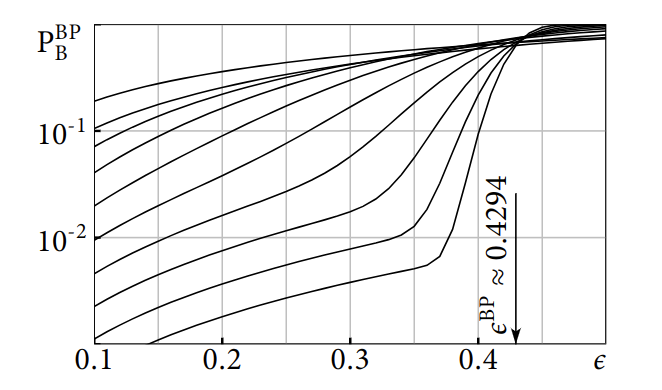
\includegraphics{performances.png} \label{fig:decoder_perf}
		\caption{Performance of decoder}
	\end{center}
\end{figure}
\section{Regular vs irregular Codes}
The Tanner graph picture makes it simple to visualize the connections between variables and check equations. If all the variable nodes have the same number of edges connected to them and so do the check nodes the code is called \textbf{regular}. Any code as a tanner graph can be the seen as having sockets attached to each node. Each socket have a number of edges facing the rest of the graph and the sockets are labelled by the number of edges they provide. See picture \ref{fig:TannerRegular} for an example. 

\begin{figure}[h]
	\begin{center}
		\begin{tikzpicture}[auto]
		\node [pinstyle] (v1) {$v_1$};
		\node [socket, right of = v1, node distance=1cm] (vs1) {};
		 		\node [pinstyle, right of = vs1] (v1_b) {};
		 		\node [pinstyle, above of =  v1_b, node distance=0.5cm] (v1_a) {};
		 		\node [pinstyle, below of = v1_b, node distance=0.5cm] (v1_c) {};
		\draw [-] (v1) -- node[name=u] {} (vs1);
			\draw [-] (vs1) -- node[name=u] {} (v1_a);
			\draw [-] (vs1) -- node[name=u] {} (v1_b);
			\draw [-] (vs1) -- node[name=u] {} (v1_c);
		
		\node [pinstyle, below of = v1, node distance=1cm] (v2){};
		\node [pinstyle, below of = v2	, node distance=2cm] (v4) {$\vdots$};
		\node [pinstyle, below of = v4, node distance=2cm] (v6) {};
		
		\node [pinstyle, below of = v6, node distance=1cm] (vn) {$v_n$};
		\node [socket, right of = vn, node distance=1cm] (vs1) {};
		\node [pinstyle, right of = vs1] (v1_b) {};
		\node [pinstyle, above of =  v1_b, node distance=0.5cm] (v1_a) {};
		\node [pinstyle, below of = v1_b, node distance=0.5cm] (v1_c) {};
		\draw [-] (vn) -- node[name=u] {} (vs1);
		\draw [-] (vs1) -- node[name=u] {} (v1_a);
		\draw [-] (vs1) -- node[name=u] {} (v1_b);
		\draw [-] (vs1) -- node[name=u] {} (v1_c); 		 		

		
		\node [pinstyle, right of=v2, node distance=6cm] (c1) {$c_1$};
			\node [socket, left of = c1, node distance=1cm] (cs1) {};
 		\node [pinstyle, left of = cs1] (c1_b) {};
 		\node [pinstyle, above of =  c1_b, node distance=0.5cm] (c1_a) {};
 		\node [pinstyle, below of = c1_b, node distance=0.5cm] (c1_c) {};
 		\draw [-] (c1) -- node[name=u] {} (cs1);
 		\draw [-] (cs1) -- node[name=u] {} (c1_a);
 		\draw [-] (cs1) -- node[name=u] {} (c1_b);
 		\draw [-] (cs1) -- node[name=u] {} (c1_c); 		 		
		
		\node [pinstyle, right of=v4, node distance=6cm] (c2) {$\vdots$};
		\node [pinstyle, right of=v6, node distance=6cm] (c3) {$c_{n-k}$};
			\node [socket, left of = c3, node distance=1cm] (csn) {};
			\node [pinstyle, left of = csn] (c1_b) {};
			\node [pinstyle, above of =  c1_b, node distance=0.5cm] (c1_a) {};
			\node [pinstyle, below of = c1_b, node distance=0.5cm] (c1_c) {};

			\draw [-] (csn) -- node[name=u] {} (c1_a);
			\draw [-] (csn) -- node[name=u] {} (c1_b);
			\draw [-] (csn) -- node[name=u] {} (c1_c); 
		
		\end{tikzpicture}
	\end{center}
	\caption{The tanner graph of a regular code}
	\label{fig:TannerRegular}
\end{figure}
Codes will not be considered as a single entity but as a family with the same degree distribution as we saw before. A family (or \textbf{ ensamble}) is then labelled by two numbers corresponding to the degree of each variable and check node respectively, $l$ and $r$. 

This parametrization through the nodes degrees $l$, $r$ is a very useful one. To get an idea, one can think about the fact that once the sockets are fixed you can connect the variable and check nodes in only a certain amount of ways. There is a constraint such that you actually are able to use up all edges form all sockets without leftovers. The constraint is very simple you count all the edges involved in the graph from the variable perspective, i.e. $nl$ and all the edges involved from the check perspective $kr$. The number of edges in the graph e is the same and constant so:
\begin{equation} 
	nl = kr
\label{eq:edge_constraint_reg}
\end{equation} 

The code rate can now be reparametrized by these two numbers and leave the total number of variables independent. So the families of codes are ensambles with a fixed R and variable n.
Using eq. \ref{eq:edge_constraint_reg}
\begin{equation}
	R = \frac{n-k}{n} = 1 -\frac{l}{r}
\end{equation} 

\section{LDPC Codes}
The most promising codes in terms of performance are the so called LDPC or Low density parity check codes. They were invented by Gallager in the sixties, but they were rediscovered and analyzed in full only in the late 1990s and 2000s. They are linear codes but with one key characteristic. The H matrix describing them is very sparse. Usually, a code is described in terms of the degree distribution of the corresponding Tanner graph. To start with, we describe a regular $(l,r)$-LDPC. It is a tanner graph where each variable and check node resp. has the same number of edges attached to it, namely $l$ and $r$. The sparsity that we where referring to in the $H$ matrix is basically the number of edges of the graph. This number is of outmost importance in decoding. This is because decoding is an algorithm that runs over the edges of the Tanner graph exchanging information between variable and check nodes. The less there are the simpler the decoding process. The better the number of edges scales with larger and larger codelength $n$, the better. Regular codes in general behave quite well, i.e. linearly as shown in eq. \ref{eq:edge_constraint_reg}. this was actually one of the reasons Gallager invented LDPC codes. They where sparse, so they had very few edges and regular, they scaled well in n. more advancement in LDPC theory and decoding put forward the idea that also irregular codes can work well (or actually better) if designed correctly. W

\section{Node and edge degree distribution}
To study more general codes, i.e irregular codes and address their performances and description one needs to generalize how we have parametrized the ensambles so far, using degrees $l$, $r$ to allow them to be variable. In an ensamble, we do not need to label precisely which node has which degree, but only count how many nodes have a specific degree and get a distribution of these frequencies. When mathematicians have these kind of problems, they resort to a massively powerful tool, generating functions. There is actually a before and after, learning about generating functions in maths as they open up a wide array of techniques to solve common problems. One of those problems is the one at hand, enumeration. 

\subsection{Node persective}
Define the variable and check degree distribution generating function (from node perspective) as:
\begin{eqnarray}
	\Lambda(x) &=& \sum_{i=1}^{d_v} \Lambda_i x^i \\
	P(x) &=& \sum_{i=1}^{d_c} P_i x^i \\
\end{eqnarray} 
where $d_v$ and $d_c$ are respectively the variable and check node max degree. In those generating functions the $x$ variable is just a bookkeeping device for the number of edges of that socket.
$\Lambda_i$ is the number of variable nodes with degree $i$. Similarly, $P_i$ is the number of check nodes with degree $i$. One can normalize the degree functions as: 
\begin{eqnarray}
L(x) &=& \frac{\Lambda(x)}{\Lambda(1)} \\
R(x) &=& \frac{P(x)}{P(1)} \\
\end{eqnarray} 

Notice that:
\begin{eqnarray}
\Lambda(1) &=& \text{Total number of variable nodes} \\
P(1) &=& \text{Total number of check nodes} \\
\Lambda^\prime(1) = P^\prime(1) &=&  \text{Total number of edges}
\end{eqnarray} 


\subsection{Edge perspective}
Define the variable and check degree distribution generating function (from edge perspective) as:
\begin{eqnarray}
\lambda(x) &=& \sum_{i=1}^{d_v} \lambda_i x^{i-1} \\
\rho(x) &=& \sum_{i=1}^{d_c} \rho_i x^{i-1} \\
\end{eqnarray} 
$\lambda_i$ is the fraction of edges connected to variable node with degree $i$. Similarly, $\rho_i$ the fraction of edges connected to check nodes with degree $i$. These are obviously automatically normalized. 
\begin{definition}[Design rate]
	\begin{eqnarray}
	R(\lambda, \rho) = 1 - \frac{\sum_i \frac{\rho}{i}}{\sum_i \frac{\lambda_i}{i}} = 1 - \frac{\int_0^1 \rho(x)dx}{\int_0^1 \lambda(x)dx}
	\end{eqnarray}
\end{definition}
This way of describing the codes we are using is very practical and of widespread use in the literature. Moreover, it is this very description in terms of generating functions that allows the code to be optimized to achieve the best performances under iterative decoders. 
Let's see some example of degree distribution.  
\subsection{Hamming code - degree distributions}
The Hamming code $\mathcal{H}(7,4)$ distributions are:
\begin{eqnarray}
	\Lambda(x) &=& 3x+3x^2+x^3, \\
	P(x) &=& 3x^4
\end{eqnarray}
the number of nodes and edges are: 
\begin{eqnarray}
 	\Lambda(1) &=& 7 \\
 	P(1) = &=& 3 \\
 	\Lambda^\prime(1) = P^\prime(1) &=& 12
\end{eqnarray}
From the node perspective
\begin{eqnarray}
\lambda(x) &=& \frac{1}{4}+\frac{1}{2}x+\frac{1}{4}x^2, \\
\rho(x) &=& x^3
\end{eqnarray}
and finally the code rate is:
\begin{eqnarray}
R = 1 - \frac{\frac{1}{4}}{\frac{1}{4} + \frac{1}{4} + \frac{1}{12}} = 1 - \frac{3}{7} = \frac{4}{7}
\end{eqnarray}
As we already know. 

We can generalize it to an arbitrary Hamming code. Let's remind that a general Humming code of codelength $n$ has a number of check nodes $k$ such that $2^k-1 = n$ or $k=\log(1+n)$. From the fact that a Hamming code $H$ matrix columns exhaust all possible sequences of bits of length $k$ apart from zero, we can convince ourselves that the edge distributions are:

\begin{eqnarray}
\Lambda(x) &=& \binom{k}{1}x+\binom{k}{2}x^2+\binom{k}{3}x^3 + \dots + \binom{k}{k}x^k, \\
P(x) &=& kx^{2^{k-1}}
\end{eqnarray}

the edge count from the second of the equations is straightforward: 
\begin{eqnarray}
\Lambda(1) &=& n \\
P(1) = &=& k \\
\Lambda^\prime(1) = P^\prime(1) &=& k2^{k-1} \label{eq:hammingexedgecount}
\end{eqnarray}

\begin{proof}
The derivative of $P$ is just immediate to do. We know that they should be equal but let us check it for completeness.

\begin{eqnarray}
	 \Lambda^\prime(1) = \sum_{j=1}^{k} j\binom{k}{j}
\end{eqnarray}
taking the derivative of the Newton binomial formula:
\begin{eqnarray}
\frac{d}{dx}(1+x)^k|_{x=1} &=& \frac{d}{dx}\sum_{j=1}^{k}\binom{k}{j}x^j \\
k2^{k-1} &=& \sum_{j=1}^{k} j\binom{k}{j} 
\end{eqnarray}
\end{proof}

The equation \ref{eq:hammingexedgecount} in terms of the codelength $n$ is:
\begin{eqnarray}
kx^{2^{k-1}} = \frac{\log(1+n)(1+n)}{2}
\end{eqnarray}

Which shows that the Humming code edge count growth is not linear. This fact, plus the density of the H matrix is bad news for its decoding performance compared to the linear regular codes.




\subsection{Regular LDPC codes - degree distributions}
The regular codes are denoted by $\mathcal{C}(n, j, l)$ where $j$ is the number of edges per variable node and $l$ is the number of edges per check node. $k$ is the number of check nodes. Obviously, $k=\frac{nj}{l}$. They are much simpler to deal with.
Their distributions in node perspective are:
\begin{eqnarray}
\Lambda(x) &=& nx^j, \\
P(x) &=& \frac{nj}{l}x^{l}
\end{eqnarray}
The number of edges is $\Lambda^\prime(1) = nj = kl$ and so it scales linearly with the codelength.


\section{Multi edge and protograph codes}
\newpage

\chapter{Message Passing Decoding}

\section{Factor graphs}

\section{Marginalization via message passing on trees}

\section{Cycles, Trees and optimality of the decoder}

\bibliographystyle{plain}
\bibliography{biblio}

\end{document}
